\documentclass[11pt]{article}
\usepackage[top = 2cm, bottom = 2cm, left = 1.5cm, right = 1.5cm]{geometry}

\usepackage[czech]{babel}
\usepackage[utf8]{inputenc}
\usepackage{graphicx}

\newcommand\qu[1]{„#1“}

\title{\Huge{J\&K Zpěvník}}
\author{\sc{Jakub Komárek \& Jiří Blaha}}
\date{}
\usepackage{ifpdf}
\usepackage[chorded]{songs}
%\renewcommand{\songlink}[2]{#2}
%\chordsoff  % Zakomentuj pro akordy
%\usepackage{fullpage}
\renewcommand{\everychorus}{\textnote{R:}}

\newindex{contentscz}{contentscz}
\newindex{contentsen}{contentsen}
\begin{document}
	\maketitle
	\thispagestyle{empty}
	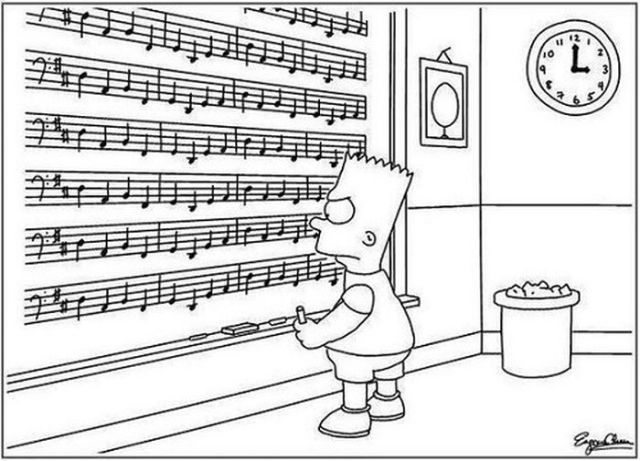
\includegraphics[width=0.9\textwidth]{cover}
	\newpage
	\songcolumns{2}
	\songpos{3}
	

	\begin{songs}{contentscz}
	\beginsong{1982}[by=Vypsaná fixa]
\beginverse      
\[E]Chlapeček \[C]brečí, \[E]nesmíš ho \[C#]hladit
\[E]Když ho budeš \[A]hladit, \[F#]tak ho můžeš \[H]zabít
\[E]Seš víla \[C]lipís, \[E]máš bílý \[C#]auto
\[E]Všechny nás \[A]vozíš a \[F#]to máme \[H]za to
\[E]že známe \[C]heslo,\[E] \[C#] 
\[E]že známe \[A]heslo,\[F#] \[H]
\[E]Li\[F]pís mi kája!\[E] \[F]
\endverse
\beginchorus
\[E]devatenátset\[D]osmdesátdva\[G] \brk- jsem malej ýmo a \[A]ty jsi princezna
\[E]devatenátset\[D]osmdesátdva\[G] \brk- nejlepší pop art, led\[A]ňáček, kofola
\[E]devatenátset\[D]osmdesátdva\[G] \brk- brutální všechno, nej\[A]lepší vzpomínky
\[E]devatenátset\[D]osmdesátdva\[G] \brk- nejlepší nohy ma\[A]minky, maminky
\endchorus
\beginverse
=1
\endverse
\beginchorus
\rep{2}
\endchorus
\endsong
\beginsong{Amazonka}[by=Hop Trop]
\beginverse
Byly krásný naše \[G]plány,
byla jsi můj celej \[Hmi]svět,\[Bmi]\[Ami]
\[Ami]čas je vzal a nechal \[G]rány,
\[Ami]starší jsme jen o pár \[D]let.
\endverse
\beginverse
Tenkrát byly děti ^malý,
ale život utí^ká,^^
^už na "táto" slyší ^jinej,
^i když si tak neří^ká.
\endverse
\beginchorus
Nebe modrý zrca\[G]dlí se
v \[E7]řece, která všechno \[Ami]ví,
stejnou barvu jako \[G]měly
\[Ami]tvoje oči džíno\[D]vý.
\endchorus
\beginverse
Kluci tenkrát, co tě znali,
všude, kde jsem s tebou byl,
"Amazonka" říkávali,
a já hrdě přisvědčil.
\endverse
\beginverse
Tvoje strachy, že ti mládí
pod rukama utíká
vedly k tomu, že ti nikdo
"Amazonka" neříká.
\endverse
\beginchorus \endchorus
\beginverse
Zlatý kráse cingrlátek,
jak sis časem myslela,
vadil možná trampskej šátek,
nosit dáls' ho nechtěla.
\endverse
\beginchorus \endchorus
\beginverse
Teď jsi víla z paneláku,
samá dečka, samej krám,
já si přál jen, abys byla
pořád stejná, přísahám,
\[Ami]pořád stejná, přísah\[G]ám.
\endverse
\endsong
\beginsong{Amerika}[by=Lucie]
\beginverse*
\[G]Nandej mi \[D]do hlavy tvý \[Ami]brouky
A Bůh nám seber bezna\[G]děj
V duši zbylo \[D]světlo z jedný \[Ami]holky
Tak mi teď za to vyna\[G]dej
Zima a \[D]promarněný \[Ami]touhy
Do vrásek stromů padá \[G]déšť
Zbejvaj roky \[D]asi ne moc \[Ami]dlouhý
Do vlasů mi zabroukej\[C]... pa pa pa \[G]pá
pa pa pa \[Emi]pá, pá pa pa \[G]pá
pa pa pa \[Emi]pá, pá pa pa \[G]pá
\endverse
\beginverse*
Tvoje oči jenom žhavý tóny
Dotek slunce zapadá
Horkej vítr rozezní mý zvony
Do vlasú ti zabrouká
pa pa pa pá, pa pa pa pá, pá pa pa pá ..
\endverse
\beginverse*
Na obloze krídla tažnejch ptáků
Tak už na svý bráchy zavolej
Na tváře ti padaj slzy z mraků
A Bůh nám sebral beznaděj
V duši zbylo světlo z jedný holky
Do vrásek stromů padá déšť
Poslední dny hodiny a roky
Do vlasů ti zabrouká...
pa pa pa pá, pa pa pa pá, pá pa pa pá... 
\endverse
\endsong
\beginsong{Andělé}[by=Wanastowi vjecy]
\beginverse
\[A]Co tě to \[E]hned po rámu na\[D]padá
\[A]nohy ruce \[E]komu je chceš \[D]dát.
\[A]Je to v krvi \[E]co tvou hlavu \[D]přepadá
\[A]chtělas padnout \[E]do hrobu a \[D]spát.
\endverse
\beginchorus
\[C]Poraněni \[G]andělé jdou do \[F]polí
\[C]stěhovaví \[G]lidi ulí\[F]taj
\[C]panenku \[G]bodni, ji to \[F]nebolí
\[C]svět je, mami, \[G]prapodivnej \[F]kraj.
\endchorus
\beginverse
Po ránu princezna je ospalá
na nebi nemusí se bát
v ulicích doba zlá ji spoutala
polykač nálezů a ztrát
\endverse
\beginchorus\endchorus
\beginverse
Co tě to zas po ránu napadá
za zrcadlem nezkoušej si lhát
miluju tě, chci tě - to ti přísahám
na kolenou lásce pomož vstát 
\endverse
\beginchorus
+ svět je mami dokonalej kraj, svět je, mami, dokonalej kraj... 
\endchorus
\endsong
%\beginsong{Antidepresivní rybička}[by=Vypsaná fixa]
\beginverse
Ona má \[C]antidepre\[Emi]sivní rybi\[F]čku
vy\[C]tetovanou na \[Emi]nejtajněšjím \[F]místě
\[C]možná je pod \[Emi]srdcem a \[F]možná trochu \[C]níž
\[C]ona muže \[Emi]všude prostě \[F]tam kam si vymyslíš
\endverse
\beginchorus
A ona \[C]plave z orgánu \[G]do orgánu
žere \[Ami]plevel kte\[D]rej po ránu
\[C]omotáva mozek a \[G]kotníky na konci pele\[Ami]sti\[D]
\endchorus
\beginchorus
A ona plave z modřiny do modřiny
a vygumuje je uplně všechny
a tvoje vnitřní orgány
tolerují tvoje rebelství
\endchorus
\beginverse
Veze si antidepresivní rybičku
městem, co má velkou spoustu pastí
falešný městský strážník
bary a zloději kol
a nebo prostě každý
koho si - ty vymyslíš
\endverse
\beginchorus
Ona je rebel, kouří na zastávce.
Jí to chutná a v týhle válce
a její vnitřní orgány
tolerují její rebelství. \rep{2}
\endchorus
\beginverse*
A potom \[C]přijde DJ \[G]Punk,
bude to \[Ami]nejlepší herec a \[D]další
a \[C]celej under\[G]ground
i ryba \[Ami]pod monopo\[D]lem \rep{2}
\endverse
\endsong
\beginsong{Batalion}[by=Spirituál Kvintet]
\beginverse*
\[Ami]Víno \[C]máš a \[G]markyt\[Ami]ánku
\[Ami]dlouhá \[C]noc se \[G]pro\[Emi]hý\[Ami]ří.
\[Ami]Víno \[C]máš a \[G]chvilku \[Ami]spánku
\[C]díky, \[G]díky \[Emi]verbí\[Ami]ři.
\endverse
\beginverse
\memorize
\[Ami]Dříve než se rozední
kapitán \[C]k osedlání \[G]rozkaz \[Ami]dá\[Emi]vá.
\[Ami]Ostruhami do slabin ko\[G]ně \[Ami]po\[Emi]há\[Ami]ní.
\[Ami]Tam na straně polední
čekají \[C]ženy, zlaťá\[G]ky a \[Ami]slá\[Emi]va.
\[Ami]Do výstřelů z karabin zvon \[G]už \[Ami]vy\[Emi]zvá\[Ami]ní.
\endverse
\beginchorus
\[Ami]Víno na ku\[C]ráž a \[G]pomilovat marky\[Ami]tánku.
\[Ami]Zítra do Bur\[C]gund bata\[G]lion \[Ami]za\[Emi]mí\[Ami]ří.
\[Ami]Víno na ku\[C]ráž a k \[G]ránu dvě hodiny \[Ami]spánku.
\[Ami]Díky, díky \[C]vám králov\[G]ští \[Ami]ver\[Emi]bí\[Ami]ři.
\endchorus
\beginverse
^Rozprášen je batalion
poslední ^vojáci se k ^zemi ^hrou^tí.
^Na polštáři z kopretin bu^dou ^věč^ně ^spát.
^Neplač sladká Marion
verbíři ^nové chlapce ^přive^dou ^ti.
^Za královský hermelín pad^ne ^kaž^dý ^rád.
\endverse
\beginchorus \endchorus
\endsong
\beginsong{Bedna od whisky}[by=Miki Ryvola] 
\beginverse
\[Ami]Dneska už mně \[C]fóry ňák \[Ami]nejdou přes py\[E]sky,
\[Ami]stojím s dlouhou \[C]kravatou na \[Ami]bedně \[E]vod whi\[Ami]sky,
\[Ami]stojím s dlouhým \[C]vobojkem \[Ami]jak stájovej \[E]pinč,
tu \[Ami]kravatu, co \[C]nosím, mi \[Ami]navlík' \[E]soudce \[Ami]Lynč.\[A]
\endverse
\beginchorus
Tak \[A]kopni do tý \[D]bedny, ať \[E]panstvo neče\[A]ká,
jsou dlouhý schody \[D]do nebe a \[E]štreka dale\[A]ká
do nebeskýho \[D]baru, já \[E]sucho v krku \[A]mám,
tak kopni do tý \[D]bedny, ať \[E]na cestu se \[A]dám.\[Ami]
\endchorus
\beginverse
Mít tak všechny bedny od whisky vypitý,
postavil bych malej dům na louce ukrytý,
postavil bych malej dům a z vokna koukal ven
a chlastal bych tam s Bilem a chlastal by tam Ben.
\endverse
\beginchorus \endchorus
\beginverse
Kdyby jsi se, hochu, jen porád nechtěl rvát,
nemusel jsi dneska na týhle bedně stát,
moh' jsi někde v suchu tu svoji whisku pít,
nemusel jsi dneska na krku laso mít.
\endverse
\beginchorus \endchorus
\beginverse
Až kopneš do tý bedny, jak se to dělává,
do krku mi zůstane jen dírka mrňavá,
jenom dírka mrňavá a k smrti jenom krok,
má to smutnej konec a whisky ani lok.
\endverse
\beginchorus
.... tak kopni do tý bedny.
\endchorus
\endsong
%\beginsong{Běž dál}[by=Poletíme]
\beginverse
\[G]Když máš hlad \[Ami]velikej,  \[Emi]tak jako \[D7]největší \[G]dům, 
když je ti \[Ami]zima, \[Emi]tak jako \[D7]severní \[G]pól, 
a nebo \[Ami]jižní, \[Emi]jen tak jsem \[D7]to sem prd\[G]nul,
zkrátka když \[Ami]bolí tě, \[Emi]že dostá\[D7]váš bum bum \[G]bum, 
\endverse
\beginchorus
Když \[C]nálada dobrá \[G]tě opustila, 
a \[Ami]všechno je černý \[G]jak černá barva, 
\[C]co se ti na pyža\[G]mu zapustila, 
\[Ami]a tvoje sny, pá pá \[D7]pá pá pá...
Běž \[G]dál, za \[Ami]každou \[Emi]zatáč\[D7]kou
můžeš \[G]potkat \[Ami]knedlík s \[Emi]omáč\[D7]kou,
běž \[G]dál, za \[Ami]nějakým \[Emi]rohem \[D7]je,
ten tvůj \[G]někdo, \[Ami]kdo tě \[G]zahře\[D7]je.
\endchorus
\beginverse
^Každý je ^silák, ^dokud ho ^něco ne^sejme, 
a pak, jak ^sirka ^hoří ^hoří sho^ří,
takhle to ^vodedá^vna už ^na světě ^je, 
tato pí^seň není ^pro ty, ^co jsou dob^ří.
\endverse
\beginchorus \endchorus
\beginverse
^Když se to ^táhne ^tak jako ^smaženej ^sýr, 
a když to ^smrdí ^jako ^zkaženej ^sýr, 
a když to má ^díry ^tak, ^jako má ^sýr, 
je to jenom sýr, ^je to sýr, ^je to sýr, ^je to jen ^sýr! 
\endverse
\beginchorus \endchorus
\endsong
%\beginsong{Buvol}[by=Vypsaná Fixa] 
\beginverse
\[Ami]Holky maj kalhoty a \[Emi]kluci šaty, \[G]je jarní \[D]den.
\[Ami]Do školy jdou a mají \[Emi]na paměti, \[G]že se rozhlí\[D]dnem.
\[Ami]Na přechodu a nebo \[Emi]jen tak kolem, \[G]dychtivě \[D]víš,  
\[Ami]jen náhlý výbuch bomby \[Emi]atomový, \[G]tě může zasta\[D]vit.
\endverse
\beginchorus 
A to je \[Ami]důvod velkej jak \[Emi]buvol,       
\[G]všichni prahnem \[D]po naději.
A to je \[C]důvod velkej jak \[G]buvol,   
na Highway to \[D]Hell.
 
\[Ami]Nanananana \[Emi]nananana
nana\[G]nánanana \[D]nánanana  
\[C]Nanananana \[G]nananau    
\[D]nananau
\endchorus
\beginverse
Holky maj kapuci a kluci rtěnky, parfém i fén,
a žlutej pyl dopadá na kapoty, aut v zácpě jen.
A všichni řidiči, kteří v nich sedí, slyší ten smích,
jen náhlá změna světel za displejem, to může zastavit.
\endverse
\beginchorus \endchorus
\beginchorus
A to je důvod, velkej jak buvol,
všichni prahnem po naději.
A to je důvod, když jedem,
po Highway to Hell.
\endchorus
\beginverse*  
\[Ami]Cesta vede z jihu na \[Emi]sever
a vyslanci z \[G]nebe nade mnou \[D]stále bdí.
\[C]Nakonec přiletíme, \[G]říka\[D]jí.
\[Ami]Cesta vede z jihu na \[Emi]sever        
a vyslanci z \[G]nebe nade mnou \[D]stále bdí.
\[C]Nakonec přiletíme, \[G]říka\[D]jí.
\endverse*
\beginchorus
A to je důvod velkej jak buvol,
á áa aa.
A to je důvod, když jedem,
po Highway to Hell.

A to je důvod velkej jak buvol,
á áa aa.
A to je důvod, když jedem,
po Highway to Hell.

\[Ami]Tam spolu jedem\[Emi]\[G] \[D]spolu je\[C]dem. \[G]\[D]                
\[Ami]Tam spolu jedem\[Emi]\[G] \[D]spolu je\[C]dem. \[G]Po Highway to \[D]Hell!
\endchorus
\endsong
\beginsong{Cesta}[by=Kryštof]\beginverse
To\[C]u cestou 
Tím směrem prý bych \[G]se dávno měl dát 
Kdy\[Am]z sněží, jde to stěží, ale sněhy pak tají 
Kus\[F] něhy ti za nehty\[G] slíbí a dají 
Víc\[C] síly se prát 
Na dne víc\[G] dávat než brát. 
A i\[Am] když se vleče a je schudná jen v kleče 
Donutí\[F] přestat se zbytečně\[G] ptát 
\endverse
\beginchorus
Jestli se \[C]blížím k cíli, kolik\[G] zbývá víry
Kam\[Am] zvou - svodidla, co po tmě mi\[F] lžou?\[G]
Snad\[C] couvám zpátky a \[G]plýtvám řádky 
C\[Am]o řvou že uz mi doma neote\[F]vřou\[G]
\endchorus
\beginverse
Nebo jít \[C]s proudem 
Na lusknutí prstu\[G] se začít hned smát, 
Mít\[Am] svuj chodník slávy a před sebou davy 
A přes\[F] zkroucená záda být\[G] součástí stáda 
Ale\[C] zpívat a hrát, kotník\[G]y líbat a stát 
Na\[Am] křídlech vsech slavíku \brk a vlastně už ze zvyku 
\[F]Přestat se zbytečn\[G]ě ptát
\endverse
\beginchorus 
\rep{2}
\endchorus
\endsong

\beginsong{Černá díra}[by=Karel Plíhal]
\beginverse
\[D]Mívali jsme \[A]dědečka, \[G]starého už \[A]pá\[D]na,
\[D]stalo se to \[A]v červenci \[G]jednou časně \[A]zrá\[D]na,
\[Hmi]šel do sklepa \[G]pro vidle, \[E]aby seno \[A]sklízel,
\[D]už se ale \[A]nevrátil, \[G]prostě někam \[A]zmi\[D]zel.
\endverse
\beginverse
Máme doma ve sklepě malou černou díru,
na co přijde, sežere, v ničem nezná míru,
nechoď, babi, pro uhlí, sežere i tebe,
už tě nikdy nenajdou příslušníci VB.
\endverse
\beginverse
Přišli vědci zdaleka, přišli vědci zblízka,
babička je nervózní a nás, děti, tříská,
sama musí poklízet, běhat kolem plotny,
a děda je ve sklepě nekonečně hmotný.
\endverse
\beginverse
Hele, babi, nezoufej, moje žena vaří
a jídlo se jí většinou nikdy nepodaří,
půjdu díru nakrmit zbytky od oběda,
díra všechno vyvrhne, i našeho děda.
\endverse
\beginverse
Tak jsem díru nakrmil zbytky od oběda,
díra všechno vyvrhla, i našeho děda,
potom jsem ji rozkrájel motorovou pilou,
opět člověk zvítězil nad neznámou silou.
\endverse
\beginverse
\[E]Dědeček se \[H]raduje, \[A]že je zase \[E]v penzi,
\[E]teď je naše \[H]písnička \[A]zralá pro re\[H]cen\[E]zi.
\endverse
\endsong
\beginsong{Colorado}[by=Kabát]
\beginverse
Táta \[G]vždycky říkal hochu žádný \[C]strachy
seš kovboj \[G]v Coloradu můžeš krávy \[D]pást
já radši \[G]utratil jsem psa a všechny \[C]prachy
do srdce \[G]Evropy já \[D]odjel v klidu \[G]krást
\endverse
\beginverse
Narvaný kapsy prsteny řetězy zlatý
tam kolem krku místní indiáni maj
a ti co nemakaj tak sou nejvíc bohatý
musím si pohnout dokavaď tam rozdávaj
\endverse
\beginchorus
Z Billa \[G]na Nováka změním si svý \[C]jméno
a až tu \[G]malou zemi celou rozkra\[D]dem. Rozkradem
tak se \[G]vrátím ve svý rodný Colo\[Emi]ra\[C]do
o tý \[G]zlatý žíle \[D]řeknu doma \[G]všem
\endchorus
\beginverse
Tam kradou všichni co okolo bydlej
šerif se na ně jenom hezky usmívá
kdyby se nesmál tak ho okamžitě zmydlej
házej mu kosti za to že se nedívá
\endverse
\beginverse
Místo krav tam nelžu vám prej pasou holky
a když jim nezaplatíš vyrazej ti dech
ale s IQ to tam nebude tak horký
místo na koních tam jezděj v medvědech
\endverse
\beginchorus
\rep{2}
\endchorus
\endsong

\beginsong{Čarodějnice z Amesbury}[by=Asonance]
\beginverse
1. Zuzana \[Dmi]byla dívka, \[C]která žila v \[Dmi]Amesbury,
s jasnýma \[F]očima a \[C]řečmi pánům \[Dmi]navzdory,
sou\[F]sedé o ní \[C]říkali, že \[Dmi]temná kouzla \[Ami]zná
a \[B]že se lidem \[Ami]vyhýbá a s \[B]ďáblem \[C]pletky \[Dmi]má.
\endverse
\beginverse       
Onoho ^léta náhle ^mor dobytek ^zachvátil
a pověr^čivý lid se ^na pastora ^obrátil,
že ^znají tu moc ^nečistou, jež ^krávy zabí^jí,
a ^odkud ta moc ^vychází, to ^každý ^dobře ^ví.
\endverse
\beginverse
Tak Zuza^nu hned před tri^bunál předvést ^nechali,
a když ji ^vedli městem, ^všichni kolem ^volali:
\qu{Už konec ^je s tvým řádě^ním, už ^nám neuško^díš,
teď ^na své cestě ^poslední do ^pekla ^pole^tíš!}
\endverse
\beginverse
Dosvědčil ^jeden sedlák, ^že zná její ^umění,
ďábelským ^kouzlem prý se ^v netopýra ^promění
a v noci ^nad krajinou ^létává pod ^černou oblo^hou,
sed^lákům krávy ^zabíjí tou ^mocí ^čarov^nou.
\endverse
\beginverse
Jiný zas ^na kříž přísa^hal, že její ^kouzla zná,
v noci se v ^černou kočku ^mění dívka ^líbezná,
je třeba ^jednou provždy ^ukončit ďá^belské řádě^ní,
a všichni ^křičeli jak ^posedlí:\qu{Na ^šibe^nici s ^ní!}
\endverse
\beginverse
Spektrální ^důkazy peč^livě byly ^zváženy,
pak z tribu^nálu povstal ^starý soudce ^vážený:
\qu{Je přece v ^knize psáno: ^nenecháš ča^rodějnici ^žít
a ^před ďáblovým ^učením budeš se ^na po^zoru ^mít!}
\endverse
\beginverse
Zuzana ^stála krásná s ^hlavou hrdě ^vztyčenou
a její ^slova zněla ^klenbou s tichou ^ozvěnou:
\qu{Pohrdám ^vámi, neznáte ^nic nežli ^samou lež a ^klam,
pro ^tvrdost vašich ^srdcí jen, jen ^pro ni ^umí^rám!}
\endverse
\beginverse
Tak vzali ^Zuzanu na ^kopec pod ši^benici
a všude ^kolem ní se ^sběhly davy ^běsnící,
a ona ^stála bezbran^ná, však s ^hlavou vztyče^nou,
zem^řela tiše ^samotná pod ^letní ^oblo^hou ...
\endverse
\endsong
%\beginsong{Čmelák}[by=Divokej Bill]
\beginverse
\[C]Žiju si jako v pohád\[G]ce, \[F]když nechci nejdu do prá\[C]ce 
venku se pasou ov\[G]ce, \[F]dělá si každá co \[C]chce 
Pošeptáš mi co Tě lá\[G]ká \[F]a to je pro čmelá\[C]ka 
co broukal si v klidu svůj \[G]part, najednou \[F]malá louka a \[C]start. 
\endverse
\beginverse
^Tak žijem jako v pohád^ce ^když nechcem nejdem do prá^ce, 
a to nechcem nik^dy ^venku se pasou krá^vy 
šeptáš co Tě lá^ká ^to je pro čmelá^ka
co broukal v klidu svůj ^part najednou ^malá louka a 
\endverse
\beginchorus
\[C]Sta\[G]rt, \[F]pro všechny první \[C]třídu...
\[C]Sta\[G]rt, \[F]pro všechny první \[C]třídu\[Ami]...
Ať se \[F]propadnu \[G]jestli\[C], \[Ami]nemám prav\[F]du tak dám \[G]fant, 
\[C]slunce Ti \[Ami]pihy \[F]na tváře \[G]kreslí a co \[C]já? \[Ami]Já nic, \[F]já muzi\[G]kant.
\endchorus
\beginverse
^Poslední dobou v le^se, ^nikdo neví kde ^jsme,
venku se pasou ^kozy, ^dělá si  každá co ^chce. 
Pošeptáš mi co Tě lá^ká, ^a to je pro čmelá^ka,
co broukal si v klidu svůj ^part, najednou ^malá louka a 
\endverse

\beginchorus
...Já nic, já muzikant.
\endchorus
\endsong
\beginsong{Čtyři slunce}[by=Vypsaná fixa]
\beginverse
\[Emi]Čtyři \[C]slunce \[G]svítěj\[D]\brk pro ra\[Emi]dost\[C] \[G] \[D] 
\[Emi]vlnov\[C]ka se \[G]zvedne\[D],\brk když má \[Emi]dost.\[C] \[G] \[D] 
A \[Emi]čtyři slunce \[C]svítěj,
li\[Ami]dem pod nima \[D]není zima.
Si \[Emi]jako malý \[C]dítě
a \[Ami]můžes začít \[D]zase znova.
\endverse
\beginchorus
Já \[Emi]vím\[C], někdy to \[Ami]nejde.\[D] \[Dsus4]
Já \[Emi]vím\[C], všechno to \[Ami]přejde.\[D] \[Dsus4] 
\endchorus
\beginverse
Čtyři slunce svítěj pro radost,
přejdu řeku, vede přes ní most.
Čtyři slunce svítěj,
lidem pod nima není zima.
Si jako malý dítě
a můžes začít zase znova.
\endverse
\beginchorus
Já vím, někdy to nejde
já vím, všechno to přejde
\endchorus
\beginverse  
Čtyři slunce svítěj pro radost,
vlnovka se zvedne, když máš dost.
Čtyři slunce svítěj,
lidem pod nima není zima.
Si jako malý dítě
a můžeš začít zase znova.
\endverse
\beginchorus
Já vím, někdy to nejde.
Já vím, všechno to přejde.
Já vím, někdy to nejde
já vím, všechno to přejde.
\endchorus
\beginverse
Čtyři slunce svítěj pro radost,
vlnovka se zvedne, když máš dost.
\endverse
\endsong
\beginsong{Dajána}[by=Zdeněk Borovec]
\beginverse
\[C]Lidé o ní \[Am]říkají, \[F]že je v lásce \[G7]nestálá,
\[C]ona zatím \[Am]potají \[F]jediného \[G7]v mysli má.
\[C]Na toho, \[Am]kdo klid jí vzal, \[F]dnem i nocí \[G7]čeká dál,
\[C]Krá\[Am]sná, \[F]bláho\[G7]vá Dajána.
\endverse
\beginverse
\[C]Ten kdo navždy \[Am]klid jí vzal \[F]odešel si \[G7]bůhví kam
\[C]Dajána má v \[Am]srdci žal, \[F]žije marným vvzpomínkám,
\[C]Předstírá-li \[Am]ve dne smích, \[F]pláče v nocích \[G7]bezesných,
\[C]Krá\[Am]sná, \[F]bláho\[G7]vá Dajána.
\endverse
\beginchorus
\[F]Srdce, které \[Fm]zastesklo si, s\[C] úsměvem teď \[C7]žal svůj nosí,
\[F]stále čeká, \[Fm]čeká dál, \[G]o, o, \[G7]o o o o o .
\endchorus
\beginverse
\[C]Ospalá jde \[Am]ulicí, \[F]nezbaví se \[G7]lásky pout,
\[C]Sny, jenž voní \[Am]skořicí, \[F]sny, jenž nelze \[G7]obejmout,
\[C]navždy bude \[Am]sama snít, \[F]nenalezne \[G7]nikdy klid.
\[C]Krá\[Am]sná, \[F]bláho\[G7]vá Dajána.
\endverse
\endsong
\beginsong{Darling}[by=Vypsaná fixa]
\beginverse
\[D]V bodu, kdy ti zmizí \[A]úplně všechno
si \[Emi]já vymyslim nejsladší \[G]pointy
\[D]někdo to neřeší, \[A]někdo pije drinky
\[Emi]někdo v tom bodu vykouří \[G]jointy
\[D]já mám rád hrdiny, \[A]kteří lezou po dně
a \[Emi]v poslední chvíli se \[G]zvednou
\[Emi]někdy taky dělám, \[A]že jsem vyřízenej
a \[Emi]je mi to úplně \[G]jedno.
\endverse
\beginverse*
Tak jsem řek
\[D]dno je dobrý \[A]na to aby \[Emi]sis ho prohlíd\[G]
\[D]dno je dobrý \[A]na to aby \[Emi]sis ho prohlíd\[G]
\endverse
\beginchorus
Tak jsem řek \[D]hej máš drobný \[A]darling
a \[Emi]ona řekla že nějaký \[G]má
a já jsem řek \[D]fajn, tak na dvě \[A]kávy
\[Emi]z automatu on nám je \[G]dá
a pak jsme šli \[D]ven a tam jsme \[A]stáli
tři \[Emi]hodiny a dvacet mi\[G]nut
a kolem byl \[D]svět, který byl \[A]správný
a s \[Emi]kelímkama z automa\[G]tu
\endchorus
\beginverse
V bodu kdy ti zmizí uplně všechno
jsem byl, tam to znám velmi
v podstatě to tam má svojí poetiku
a originální genius loci
lítají tam pořad ty samý bumerangy, který se pokaždý vrátěj
uprostřed toho všeho mezi strážnou věží
a pornografickým stánkem
jsem řek
dno je dobrý na to aby sis ho prohlíd
dno je dobrý na to aby sis ho prohlíd
\endverse
\beginchorus
Tak jsem řek hej smím prosit darling
a ona řekla, že jsem to já
a já sem řek fajn tak je to správný
dr. Jekyll zvítězí rád
a pak jsem řek hey, chtěl bych tě darling
a ona řekla co bude dál
hráli jsem squash a taky curling
uklízet a zaparkovat 
\endchorus
\beginverse*  
A tak jsem řek hej - to bude dál
a pak jsem řek hej - ale je tu i Hyde
a tak jsem řek hej - to bude dál
a pak jsem řek hej - ale je tu i Hyde
\endverse
\endsong
\beginsong{Detaily}[by=Vypsaná fixa]
\beginverse
\[Hmi]Město je horký, srpnový,
\[G]že v srdci taje to takový
\[D]nejvíc a nejhůř studený \[A]místo.
\[Hmi]Spící sopky se probudí,
\[G]byl dlouho pryč, kolem a v okolí.
\[D]Teď toužil a chtěl cítit \[A]blízkost.
\endverse
\beginverse*
^Čau, mami! Tak jsem tady zas.
^Jsem agent Cooper – dám si koláč.
^Hážu kříž na zem – hlavu mám ^nízko.
\endverse
\beginchorus
Mezi \[Hmi]ním mezi ní byly detaily
a kusy \[G]rodiny, který se rozpadly.
Byl to \[D]šílenej horor – řev a taky \[A]vřískot.
Mezi \[Hmi]ním mezi ní byly detaily
a kusy \[G]koláče, který dopadly
na \[D]ubrus a na zem, ale na stole bylo \[A]čisto.
\endchorus
\beginverse
Noci jsou vlahý a takový,
že srdce buší hladový,
cítíš to v sobě a víš to.
Hrdinové nekecaj a jdou
tam, kam nechce vůbec nikdo –
na nejvíc a nejhůř studený místo.
\endverse
\beginverse*
Čau, lidi! Tak jsem tady zas.
Jsem agent Cooper a jdu po vás.
Prostě to najdu – už jsem blízko.
\endverse
\beginchorus
Mezi ním mezi ní byly detaily
a kusy líčidel, který dopadly
na ubrus a na zem, ale po pláči bylo čisto.
\rep{2}
\endchorus
\beginverse*
Bolí to dlouho,
bolí to dál.
Bolí to dlouho.
Vzal za tu zataženou roletu
a vstal.
\endverse
\beginchorus
Mezi ním mezi ní byly detaily
a kusy líčidel, který dopadly
na ubrus a na zem, ale po pláči bylo čisto.
\rep{2}
\endchorus
\beginverse*
Hrdinové nekecaj a jdou do tmy.
Hrdinové nekecaj a jdou tam, kam nechce nikdo.
\rep{4}
\endverse
\endsong
\beginsong{Dezolát}[by=Vypsaná fixa]
\beginverse
\[Emi]Ty si pěkný \[C]dezolát \[D]řekla „Halí\[A]belí“
a byla to pohoda třeba se to povede
vytáhnem tvý múzy a hodíme je za tebe
kdo ty múzy zachytí ten bude mít záruku
opravdový kvality ty si pěkný dezolát
tohle řekla ona musíme tě sledovat.
\endverse
\beginchorus
\[C]A celý \[Emi]prostor je sledovaný
\[C]příjemnými \[Emi]lidmi kteří olizují
\[C]šťávu \[Emi]tekoucí
z konečků \[D]prstů.
\endchorus
\beginverse
Ty jsi pěkný dezolát, ve sprchovým koutě
teče voda ledová, třeba se to povede
opláchnu svý múzy a vypustím je pod sebe,
kdo ty múzy zachytí, ten bude mít záruku
opravdový kvality, ty si pěkný dezolát
tohle řekla ona
\endverse
\beginchorus  \endchorus
\beginverse*
\[Emi]Pustíme si \[C]starý gramofon
\[D]budeme mít \[A]světy který nás zajímají
vinylový bůh je šampion
proležíme v posteli celou neděli
pustíme si starý gramofon
budeme mít světy který nás zajímají
vinylový bůh je šampión
venku ten náš svět sledují kamery

A hudba hraje dál

Pustíme si starý gramofon
budeme mít světy který nás zajímají
vinylový bůh je šampion
venku ten náš svět sledují kamery

\[Emi]Jsem z \[C]toho celej \[A]žhavej 
\endverse
\endsong
\beginsong{Divoké koně}[by=Jaromír Nohavica]
\beginverse
\lrep \[Ami]Já viděl \[Dmi]divoké \[Ami]koně, \[C]běželi \[Dmi]soumra\[Ami]kem,\rrep
\[Dmi]vzduch \[Ami]těžký \[Dmi]byl a divně \[Ami]voněl \[G#dim]tabá\[F]kem,
\[Dmi]vzduch \[Ami]těžký \[Dmi]byl a divně \[Ami]voněl \[E7]tabá\[Ami]kem.
\endverse
\beginverse
\lrep Běželi, běželi bez uzdy a sedla krajinou řek a hor,\rrep
\lrep sper to čert, jaká touha je to vedla za obzor? \rrep
\endverse
\beginverse
\lrep Snad vesmír nad vesmírem, snad lístek na věčnost,\rrep
\lrep naše touho, ještě neumírej, sil máme dost.\rrep
\endverse
\beginverse
\lrep V nozdrách sládne zápach klisen na břehu jezera,\rrep
\lrep milování je divoká píseň večera.\rrep
\endverse 
\beginverse
\lrep Stébla trávy sklání hlavu, staví se do šiku,\rrep
\lrep král s dvořany přijíždí na popravu zbojníků.\rrep
\endverse
\beginverse
\lrep Chtěl bych jak divoký kůň běžet běžet,nemyslet na návrat\rrep
\lrep s koňskými handlíři vyrazit dveře, to bych rád.\rrep
Já viděl divoké koně ...
\endverse

\endsong
\beginsong{Dokud se zpívá}[by=Jaromír Nohavica]
\beginverse
Z\[C] Těšína \[Emi]vyjíždí \[Dmi7]vlaky co \[F]čtvrthodi\[C]nu, \[Emi]\[Dmi7]\[G]
\[C]včera jsem \[Emi]nespal a \[Dmi7]ani dnes \[F]nespoči\[C]nu, \[Emi]\[Dmi7]\[G]
\[F]svatý \[G]Medard, můj pa\[C]tron, ťuká si na če\[G]lo,
ale \[F]dokud se \[G]zpívá, \[F]ještě se \[G]neumře\[C]lo.\[Emi]\[Dmi7]\[G]
\endverse
\beginverse
^Ve stánku ^koupím si ^housku a ^slané ty^čky, ^^^
^srdce mám ^pro lásku ^a hlavu ^pro písni^čky, ^^^
^ze školy ^dobře vím, ^co by se dělat mě^lo,
ale ^dokud se ^zpívá, ^ještě se ^neumře^lo. ^^^
\endverse
\beginverse
^Do alba ^jízdenek ^lepím si ^další jed^nu, ^^^
^vyjel jsem ^před chvílí, ^konec je v^ nedohled^nu, ^^^
^za oknem ^míhá se ^život jak lepore^lo,
ale ^dokud se ^zpívá, ^ještě se ^neumře^lo. ^^^
\endverse
\beginverse
^Stokrát jsem ^prohloupil ^a stokrát ^platil dra^ze, ^^^
^houpe to, ^houpe to ^na housen^kové drá^ze, 
^i kdyby ^supi se ^slítali na mé tě^lo,
tak ^dokud se ^zpívá, ^ještě se ^neumře^lo. ^^^
\endverse
\beginverse
Z ^Těšína ^vyjíždí ^vlaky až ^na kraj svě^ta, ^^^
^zvedl jsem ^telefon ^a ptám se: ^Lidi, jste ^tam?                
A ^z veliké ^dálky ^do uší mi zazně^lo,
\lrep že ^dokud se ^zpívá, ^ještě se ^neumře^lo. ^^^ \rrep
\endverse
\endsong
%\beginsong{Dva havrani}[by=Asonance]
\beginverse
\[Dmi]Když jsem se z pole \[C]vrace\[Dmi]la,
dva havrany jsem \[C]slyše\[Dmi]la,
\[C]jak jeden d\[F]ruhého se \[C]ptá:
\[Dmi]kdo dneska veče\[C]ři nám \[Dmi]dá?
\[Dmi]kdo dneska veče\[C]ři nám \[Dmi]dá?
\endverse
\beginverse
Ten první k druhému se otočil
a černým křídlem cestu naznačil,
krhavým zrakem k lesu hleděl
a takto jemu odpověděl
a takto jemu odpověděl:
\endverse
\beginverse
"Za starým náspem, v trávě schoulený
tam leží rytíř v boji raněný,
a nikdo neví, že umírá,
jen jeho kůň a jeho milá.
Jen jeho kůň a jeho milá."
\endverse
\beginverse
"Jeho kůň dávno po lesích běhá
a jeho milá uŽ jiného má,
už pro nás bude dosti místa,
hostina naše už se chystá.
Hostina naše už se chystá."
\endverse
\beginverse
"Na jeho bílé tváře usednem
a jeho modré oči vyklovem,
a až se masa nasytíme,
z vlasů si hnízdo postavíme.
Z vlasů si hnízdo postavíme." 
\endverse
\endsong
\beginsong{Gastrosexuál}[by=Wohnout]
\beginverse
\[F#mi]Můj doktor sebou \[E]sek a \[H]málem to neu\[F#mi]stál.
Víš, já mu tehdy \[E]řek, že \[H]jsem gastrosexu\[F#mi]ál.
Ale jen co se z lehu \[E]zved, \[H]přísně se zazu\[F#mi]bil.
Blíž jsem si k němu \[E]sed a \[H]všechno mu vyklo\[D]pil.
\endverse
\beginchorus
Do \[Hmi]příboru se oša\[E]tím a nebude mi \[F#mi]zima,\[D]
\[Hmi]stříknu pivo na ru\[E]kávy a kolu do ga\[F#mi]tí,\[E]
\[Hmi]vzít si boty z kavi\[E]áru není volo\[F#mi]vina,\[D]
na \[Hmi]léto si pak uva\[E]řím šaty kopro\[F#mi]vý.
\endchorus
\beginverse
^Doktor řek, no pane ^Homola, ^tím ste mě zasko^čil.
Přemýšlím stále ^dokola, ^čím bych vás vylé^čil.
S tou tváří vaší nevi^nnou ^já bych nemaro^dil.
Zkuste svůj úlet ^rozvinout, ^Doktor mi pora^dil.
\endverse
\beginchorus
Do \[Hmi]příboru se oša\[E]tím a nebude mi \[F#mi]zima,\[D]
\[Hmi]stříknu pivo na ru\[E]kávy a kolu do ga\[F#mi]tí,\[E]
\[Hmi]vzít si boty z kavi\[E]áru není volo\[F#mi]vina,\[D]
na \[Hmi]léto si pak uva\[E]řím šaty kopro\[F#mi]vý
a gu\[E]lášo\[H]vý fi\[F#mi]ží.
Noha\[F#mi]vičky z marci\[E]pánu s vanil\[H]kovou příchu\[F#mi]tí.
\[F#mi]Šál maza\[E]ný bruše\[H]tou z tymi\[F#mi]ánu
a knoflíky ze sa\[E]lámu kula\[H]ťoučký vykro\[D]jím.
\endchorus
\beginverse*
Na na náj..
\endverse
\beginchorus \endchorus
\endsong

\beginsong{Hej teto!}[by=Michal Horák]
\beginverse
Měl jsem \[Ami]hlídat tetě \[C]křečka,
\[G]dala mi ho se slovy,
ať \[D]u mě chvíli přečká.

Ale křečka uhlídati
nelze jen tak lehce, 
obzvlášť když se vám moc nechce.

Po pokoji ať si  běhá,
na gauč jsem si lehnul,
vzápětí se ani nehnul.

Tlačilo mě do zad kromě
polštářů i cosi,
už se vidím tetu prosit:
\endverse
\beginchorus
Hej \[F]teto, já ho \[C]zabil,
\[E]už se to nestane, jo
\[Ami]ten už asi nevstane.
Hej \[F]teto, nekřič \[C]na mě,
\[E]já ho prostě neviděl,
\[Ami]už dost jsem se nastyděl,
hej \[F]teto!

\[C] \[E] \[Ami] \[F] \[C] \[E] \[E7]
\endchorus
\beginverse
Tak jsem kouknul,co mě tlačí,
seděl jsem jenom 
na televizním ovladači,

ale křeččí švitoření
slyšet není, jenom
zvláštní smrad se line od topení.

Zase se mi dech zatajil,
spečeného křečka
bych před tetou neobhájil.

A dřív než tam sebou seknu,
měl bych asi vymyslet,
jak tetě potom řeknu:
\endverse
\beginchorus \endchorus
\beginchorus
Hej teto,
já ho fakt zabil,
ten bídák sežral magnet
a k topení se přitavil.

Hej teto,
co na to říci?
Můžeš si ho maximálně připnout na lednici.
\endchorus
\beginchorus  \endchorus


\endsong

\beginsong{Hlídač Krav}[by=Jaromír Nohavica]\beginverse
K\[C]dyž jsem byl malý, říkali mi naši:
"Dobře se uč a jez chytrou kaši,
\[F]až jednou vyrosteš, b\[G]udeš doktorem pr\[C]áv,
takový doktor sedí pěkně v suchu,
bere velký peníze a škrábe se v uchu,"
\[F]já jim ale na to řek':Ch\[G]ci být hlídačem k\[C]rav.
\endverse
\beginchorus
Já chci \[C]mít čapku s bambulí nahoře,
jíst kaštany a mýt se v lavoře,
\[F]od rána po celý d\[G]en zpívat si j\[C]en,
zpívat si: pam pam pa\[F]m \[G]..\[C].
\endchorus
\beginverse
K vánocům mi kupovali hromady knih,
co jsem ale vědět chtěl, to nevyčet' jsem z nich:
nikde jsem se nedozvěděl, jak se hlídají krávy,
ptal jsem se starších a ptal jsem se všech,
každý na mě hleděl jako na pytel blech,
každý se mě opatrně tázal na moje zdraví.
\endverse
\beginchorus  \endchorus
\beginverse
Dnes už jsem starší a vím, co vím,
mnohé věci nemůžu a mnohé smím,
a když je mi velmi smutno, lehnu si do mokré trávy,
s nohama křížem a s rukama za hlavou
koukám nahoru na oblohu modravou,
kde se mezi mraky honí moje strakaté krávy.
\endverse
\beginchorus  \endchorus
\endsong

\beginsong{Hodinový hotel}[by=Mňága \& Žďorp]
\beginverse
 \[C]Tlusté koberce plné \[Emi]prachu
 \[A]poprvé s holkou, \[F]trochu \[G]strachu
 \[C]a stará dáma od vedle zas \[Emi]vyvádí
 \[A]zbyde tu po ní zvadlé \[F]kapradí
a pár \[G]prázdných flašek
\[C]veterán z legií n\[Emi]adává na revma
\[A]vzpomíná na Emu, \[F]jak byla \[G]nádherná
a \[C]všechny květináče už tu historku \[Emi]znají,
ale \[A]znova listy nakloní a poslou\[F]chají
vzduch voní \[G]kouřem.
\endverse
\beginchorus
\[C]a svět je, \[Emi]svět je jenom hodinový \[A]hotel
a můj \[F]pokoj je \[G]studený a \[C]prázdný
\rep{2}
\endchorus
\beginverse
Vezmu si sako a půjdu do baru
absolventi kurzu nudy, pořád postaru
kytky v klopě vadnou, dívám se okolo po stínech:
Kterou? No přeci žádnou!
vracím se pomalu nahoru
cestou potkávám ty, co už padají dolů
a vedle v pokoji někdo šeptá:"Jak ti je?"
za oknem prší a déšť stejně nic nesmyje...
\endverse
\beginchorus  
\endchorus


\endsong

\beginsong{Hruška}[by=Čechomor]\beginverse
\[A] Sto\[D]jí hruška v širém poli
vršek se jí zelená
\lrep Pod ní se pase kůň vraný
pase ho má milá \rrep
\endverse
\beginverse
Proč \[D]má milá dnes \[A]pasete
z ve\[D]čera  \[G]do rán\[A]a
\lrep Kam \[D]můj mi\[G]lý poj\[A]ede\[D]te
já poje\[A]du s vá\[D]ma \rrep
\endverse
\beginverse
Ó \[D]já pojedu  \[A]daleko
přes  \[D]vody  \[G]hlubo\[A]ké
\lrep Kéž \[D]bych byl \[G]nikdy  \[A]nepozn\[D]al
panny čer\[A]noo\[D]ké \rrep
\endverse
\endsong

\beginsong{Hudsonský šífy}[by=Wabi Daněk]
\beginverse
\[Ami]Ten, kdo nezná hukot vody lopat\[C]kama vířený
jako \[G]já, jó jako \[Ami]já,
kdo Hud\[Ami]sonský slapy nezná sírou \[G]pekla sířený,
ať se na \[Ami]Hudsonský \[G]šífy najmout \[Ami]dá, \[G]jo-ho-\[Ami]ho.
\endverse
\beginverse
Ten, kdo nepřikládal uhlí, šíf když na mělčinu vjel,
málo zná, málo zná,
ten, kdo neměl tělo ztuhlý, \brk až se nočním chladem chvěl,
ať se na Hudsonský šífy najmout dá, johoho.
\endverse
\beginchorus
\[F]Ahoj, páru tam \[Ami]hoď,
ať \[G]do pekla se dříve dohra\[Ami]bem,
\[G]jo-ho-\[Ami]ho, \[G]jo-ho-\[Ami]ho.
\endchorus
\beginverse
Ten, kdo nezná noční zpěvy zarostenejch lodníků
jako já, jó jako já,
ten, kdo cejtí se bejt chlapem, umí dělat rotyku,
ať se na Hudsonský šífy najmout dá, johoho.
\endverse
\beginverse
Ten, kdo má na bradě mlíko, \brk kdo se rumem neopil,
málo zná, jó málo zná,
kdo necejtil hrůzu z vody, kde se málem utopil,
ať se na Hudsonský šífy najmout dá, johoho.
\endverse
\beginchorus \endchorus
\beginverse
Kdo má roztrhaný boty, kdo má pořád jenom hlad
jako já, jó jako já,
kdo chce celý noci čuchat pekelnýho vohně smrad,
ať se na Hudsonský šífy najmout dá, johoho.
\endverse
\beginverse
Kdo chce zhebnout třeba zejtra, \brk komu je to všechno fuk,
kdo je sám, jó jako já,
kdo má srdce v správným místě, \brk kdo je prostě príma kluk,
ať se na Hudsonský šífy najmout dá, johoho.
\endverse
\beginchorus
Ahoj, páru tam hoď,
ať do pekla se dříve dohrabem,
\[G]jo-ho-\[Ami]ho, \[G]jo-ho-\[Ami]ho, \[G]jo-ho-\[A]ho
\endchorus
\endsong
\beginsong{Husličky}[by=Vlasta Redl]
\beginverse
\[C]Čiže ste husličky \[F]či\[C]e
\[Dm]Kdo vás tu \[Am]zanech\[G]al \rep{2}
\[Dm]Na trávě \[G]pová\[C]lané
\[Dm]Na trávě \[G]povál\[C]ané\[F]
\[Dm]U paty\[Am] oře\[G]cha \[Dm]\[Am]\[G]
\endverse
\beginverse
\[C]Kdože tu trávu tak \[F]zvá\[C]lal
\[Dm]Aj modré \[Am]fia\[G]ly \rep{2}
\[Dm]Že ste hu\[G]sličky \[C]samé
\[Dm]Že ste hu\[G]sličky \[C]samé\[F]
\[Dm]Na světě \[Am]zosta\[G]ly \[Dm]\[Am]\[G]
\endverse
\beginverse
\[C]Který tu muzikant us\[F]nul\[C]
\[Dm]A co sa mu \[Am]přišlo \[G]zdát \rep{2}
\[Dm]Co sa mu \[G]enem \[C]zdálo
\[Dm]Bože Co sa mu \[G]enem \[C]zdálo\[F]
\[Dm]Že už vjec \[Am]nechtěl \[G]hrát \[Dmi]\[Am]\[G]
\endverse
\beginverse
\[C]Zahrajte husličky \[F]sa\[C]my
\[Dm]Zahrajte \[Am]zvese\[G]la \rep{2}
\[Dm]Až sa ta \[G]bude \[C]trápit
\[Dm]Až sa ta \[G]bude \[C]trápit\[F]
\[Dm]Která ho \[Am]nechtě\[G]la \[Dm]\[Am]\[G]
\endverse
\endsong

%\beginsong{Chci tančit}[by=Mirai]
\beginverse
\[D]Život plyne dál
\[G]Nechci promarnit ho v jistotách
\[Hmi]Než bych na břehu stál
\[Asus4]Radši stokrát bych si \[A]na dno sáhl
\[D]Ah, \[G]Sám si píšu scénář svého osudu
\[Hmi] Ah, \[Asus4]A věř mi dokud dýchám, \[A]jen komparz nebudu
\endverse
\beginchorus
Chci \[G]tančit zimou i \[D]létem,
projít \[Asus4]bez starostí celým \[Hmi]širým světem\[A].
Večer pít \[G]víno, na nebe se \[D]dívat,
počítat \[Asus4]hvězdy dokud nezačne \[Hmi]svítat\[A].
Já chci \[G]tančit zimou i \[D]létem,
projít \[Asus4]bez starostí celým \[Hmi]širým světem\[A].
Večer pít \[G]víno, na nebe se \[D]dívat.
\[A]Dokud budu jenom trochu \[G]vnímat.
\endchorus
\beginverse
\[A]Vždyť teď je \[G]tady a zítra je v \[D]dálce,
včera už tu \[A]bylo, tak mi dovol \[Asus4]smát se\[A].
Tak nech mě jenom \[G]dýchat, na chvíli běž.
Dej si klidně \[A]na čas, jestli chceš.\[Asus4]\[A]
Já nechci ten \[G]závod, já chci jen \[D]žít.
A zpívat si \[A]dokola si na celý byt.\[Asus4]\[A]
\[G]\[D]\[A]
\endverse
\beginchorus  \endchorus
\beginverse*
Woh\[G]ooho\[D]u \[A]wooho\[Hmi]u \[G]woo\[D]hou\[A] \rep{2}
\endverse
\beginchorus
Já chci tančit zimou i létem,
projít bez starostí celým širým světem.
Večer pít víno, na nebe se dívat.
Dokud budu jenom trochu vnímat...
\endchorus
\endsong

\beginsong{I cesta může být cíl}[by=Mňága a Žďorp]
\beginverse
\[F]Zrychlený \[C]vlak náhle \[B]stojí
\[F]asi ta\[C]k v půli \[B]cesty,
\[F]zbývá vzdát \[C]čest padlému \[B]stroji
\[F]a \[C]zbytek dojít \[B]pěšky.
\endverse
\beginverse
A náhle už není, kam spěchat,
vítací výbory nebudou čekat,
kufry a příbory tu můžeme nechat,
až déšť se vsákne, tak vystoupí řeka.
\endverse
\beginchorus
I \[F]cesta \[C]může být \[B]cíl,
I \[F]cesta \[C]může být \[B]cíl.
\endchorus
\beginverse
Jediný mrak nad hlavou stojí
nehybně, tak jako vážky,
jediný klas dozrává v poli
jediným způsobem lásky.
\endverse
\beginverse
A náhle už není, kam spěchat,
vítací výbory nebudou čekat,
kufry a příbory tu můžeme nechat,
až déšť se vsákne, tak vystoupí řeka.
\endverse
\beginchorus \endchorus
\endsong
\beginsong{Jdem zpátky do lesů}[by=Pavel Lohonka Žalman]
\beginverse
\[Am7]Sedím na kolejích, \[D7]které nikam neved\[G]ou,\[C]\[G]
\[Am7]koukám na kopretinu, jak \[D7]miluje se s lebedou\[G],
\[Am7]mraky vzaly slunce \[D7]zase pod svou ochranu\[G],ochra\[Em]nu
\[Am7]jen ty nejdeš, holka zlatá, \[D]kdypak já tě dostanu\[G]?\[D7]
\endverse
\beginchorus
Z \[G]ráje, my vyhnaní z rá\[Em]je,
kde není už m\[Am7]ísta, \[C7]prej něco se ch\[G]ystá, ó\[D]
z \[G]ráje nablýskaných ple\[Em]sů
jdem zpátky do le\[Am7]sů \[C7]za nějaký ča\[G]s\[D7].
\endchorus
\beginverse
\[Am7]Vlak nám včera ujel \[D7]ze stanice do ne\[G]be,\[C]\[G]
\[Am7]málo jsi se snažil, \[D7]málo šel jsi do sebe\[G],
\[Am7]šel jsi vlastní cestou, a \[D7]to se zrovna neno\[G]sí,\[Em]
\[Am7]i pes, kterej chce přízeň, napřed \[D]svýho pána popro\[G]sí.\[D7]
\endverse
\beginchorus  \endchorus
\beginverse
\[Am7]Už tě vidím z dálky, jak \[D7]máváš na mě koru\[G]nou,\[C]\[G]
\[Am7]a jestli nám to bude stačit, \[D7]zatleskáme na druhou\[G],
\[Am7]zabalíme všechny, co si \[D7]dávaj' rande za bra\[G]nou,\[Em]
\[Am7]v ráji není místa, možná \[D]v pekle se nás zasta\[G]nou.\[D7]
\endverse
\beginchorus  \endchorus
\endsong
\beginsong{Jelen}[by=Jelen]
\beginverse
\[Dmi]Na jaře se vrací \[C]od podzima listí.
\[Dmi]Mraky místo ptáků \[C]krouží nad závistí.
\[Dmi]Kdyby jsi se někdy \[C]ke mně chtěla vrátit,
\[Dmi]nesměla bys, lásko, \[C]moje srdce ztra\[G]tit.
\endverse
\beginchorus
\[Dmi]Zabil jsem v lese \[C]jele\[F]na.
Bez nenávisti, \[C]bez jmé\[Dmi]na.
Když přišel dolů k \[C]řece \[F]pít,
krev teče do vody, \[C]v srdci \[Dmi]klid.
\endchorus
\beginverse
Voda teče k moři, po kamenech skáče,
jednou hráze boří, jindy tiše pláče. 
Někdy mám ten pocit, i když roky plynou.
Že vidím tvůj odraz dole pod hladinou.
\endverse
\beginchorus  \endchorus
\beginverse
na jaře se vrací, listí od podzima.
Čas se někam ztrácí, brzo bude zima.
Svět přikryje ticho, tečka za příběhem.
Kdo pozná, čí kosti, zapadaly sněhem.
\endverse
\beginchorus  \endchorus
\beginchorus
\[Emi]Zabil jsem v lese \[D]jele\[G]na.
Bez nenávisti, \[D]bez jmé\[Emi]na.
Když přišel dolů k \[D]řece \[G]pít,
krev teče do vody, v \[D]srdci \[Emi]klid. 
\endchorus

\endsong

\beginsong{Karavana mraků}[by=Karel Kryl]
\beginverse      
\[D]Slunce je zlatou skobou \[Hmi]na vobloze přibitý,
\[G]pod sluncem \[A]sedlo kože\[D]ný,\[A7]
\[D]pod sedlem kůň, pod koněm \[Hmi]moje boty rozbitý
\[G]a starý \[A]ruce sedře\[D]ný.
\endverse
\beginchorus
\[D7]Dopředu \[G]jít s tou \[A]karavanou \[Hmi]mraků,
schovat svou \[G]pleš pod \[A]stetson děra\[Hmi]vý,
\lrep jen kousek \[Emi]jít, jen \[A7]chvíli, \[Hmi]do soumraku,\[Emi]
až tam, kde \[Hmi]svítí město, \[F#]město bělavý\[Hmi].\[D7] \rrep
\endchorus
\beginverse
Vítr si tiše hvízdá po silnici spálený,
v tom městě nikdo nezdraví,
šerif i soudce - gangsteři, voba řádně zvolení
a lidi strachem nezdraví.
\endverse
\beginverse
Sto cizejch zabíječů s pistolema skotačí
a zákon džungle panuje,
provazník plete smyčky, hrobař kopat nestačí
a truhlář rakve hobluje.
\endverse
\beginchorus
\[D7]V městě je \[G]řád a\[A] pro každého \[Hmi]práce,
buď ještě \[G]rád, když \[A]huba voně\[Hmi]mí,
\lrep může tě \[Emi]hřát, že \[A7]nejsi \[Hmi]na voprátce\[Emi]
nebo že \[Hmi]neležíš pár \[F#]inchů pod \[Hmi]zemí.\[D7] \rrep
\endchorus
\beginverse 
=1.
\endverse     
\beginchorus
\[D7]Pryč odtud \[G]jít s tou \[A]karavanou \[Hmi]mraků,
kde tichej \[G]dům a\[A] pušky reza\[Hmi]vý,
\lrep orat a \[Emi]sít od \[A7]rána \[Hmi]do soumraku\[Emi]
a nechat \[Hmi]zapomenout \[F#]srdce bola\[Hmi]vý.\[D7] \rrep
\endchorus
\endsong

%\beginsong{Každý Ráno}[by=Chinaski]\beginverse
\[G]Každý ráno když si \[D]vzpomenu
\[F]vzpomenu si \[C]na to jak měl jsem tě \[G]rád
a nevzal si tě \[D]za ženu
\[F]každý ráno \[C]budu si vyč\[G]ítat
jak to bylo \[D]zbabělé
\[F]když jsem na svý cestě \[C]nezdvihl tvůj drah\[G]okam
a od tý doby od \[D]čerta k ďáblu
\[F]se po tý \[C]cestě potlou\[G]kám
\endverse
\beginverse*
\[A]
\[Bm]lás--\[A]ko
jedi\[G]ná\[A]
\[Bm]lás--\[A]ko
\endverse\beginverse
\[G]
\[D]Každý ráno když si \[A]vzpomenu
\[C]vzpomenu si \[G]na to jak měl jsem tě \[D]rád
a nevzal si tě \[A]za ženu
\[C] každý ráno
\[G]budu se prokl\[D]ínat
já vůl j\[A]á blázen
\[C]kdo postaví \[G]mé nohy na zem
\[D]kdo to \[A]pro mě kromě \[C]tebe udě\[G]lá
\endverse
\beginverse
Jednou ráno až si \[D]vzpomeneš
\[F]pošli mi \[C]prosím adre\[G]su
ať mé noční můry \[D]zaženeš
\[F]ať strachy \[C]o tebe se netře\[G]su
Slibuju v příštím \[D]životě
\[F]podruhý \[C]stejnou chybu neudě\[G]lám
ať chceš nebo ne já \[D]najdu tě
\[F]a zvednu \[C]tvůj draho\[G]kam
\endverse
\beginverse*
\[D]Všechna má \[F]rána jsou prázdná
\[C]a v nedohlednu \[G]šťastný konec příbě\[D]hu
příběhu \[F]starýho blázna
\[C]co vyměnil \[G]pýchu za něhu
\endverse\endsong

\beginsong{Když mě brali za vojáka}[by=Jaromír Nohavica]
\beginverse
\[Ami]Když mě brali za vo\[C]jáka
\[G]stříhali mě doho\[C]la.
\[Dmi]Vypadal jsem jako \[Ami]blbec
\[E]Jak ti všichni doko\[F]la,
\[G]la, \[C]la, \[G]la, \[Ami]jak ti všichni \[E]doko\[Ami]la.
\endverse
\beginverse
^Zavřeli mě do ka^sáren,
^začali mě uči^ti
^jak mám správný voják ^býti
^a svou zemi chráni^ti,
^ti, ^ti, ^ti ^a svou zemi ^chráni^ti
\endverse
\beginverse
^Na pokoji po ve^čerce
^ke zdi jsem se přitu^lil.
^Vzpomněl jsem si na svou ^milou
^krásně jsem si zabu^lil,
^lil, ^lil, ^lil ^krásně jsem si ^zabu^lil
\endverse
\beginverse
^Když přijela po půl ^roce,
^měl jsem zrovna zápal ^plic,
^po chodbě furt někdo ^chodil,
^tak nebylo z toho ^nic,
^nic, ^nic, ^nic ^tak nebylo ^z toho ^nic.
\endverse
\beginverse
^Neplačte, vy oči ^moje,
^ona za to nemo^hla,
^mladá holka lásku ^potřebuje,
^tak si k lásce pomo^hla,
^hla, ^hla, ^hla ^tak si k lásce ^pomo^hla
\endverse
\beginverse
^Major nosí velkou ^hvězdu,
^před branou ho potka^la.
^Řek jí, že má zrovna ^volný kvartýr
^Tak se sbalit necha^la,
^la ^la, ^la ^tak se sbalit ^necha^la.
\endverse
\beginverse
^Co je komu do vo^jáka,
^když ho holka zradi^la.
^Na shledanou, pane ^Fráňo Šrámku,
^písnička už skonči^la.
^La, ^la, ^la, ^jakpak se Vám ^líbi^la?
\[G]La, \[C]la, \[G]la, \[Ami]nic moc extra \[E]neby\[Ami]la... 
\endverse
\endsong
\beginsong{Klára}[by=Chinaski]
\beginverse*
\[H]Ná nananan\[G#mi]nananananana \[E]ná \[Emi]
\[H]Ná nananan\[G#mi]nananananana \[E]ná \[Emi]
\endverse
\beginverse*
\[H]Kláro, jak to s \[D#mi]tebou vypadá
od půl \[C#mi]devátý, do osmi \[Emi]ráno
Co nám \[H]brání bejt spolu \[D#mi]jenom ty a já
Nebuď \[C#mi]včerejší no tak \[Emi]Kláro
\endverse
\beginverse*
Pro tebe \[H]slibuju, žaluju denně \[D#mi]piju jak Dán
\[C#mi]ve skrytu duše marně \[Emi]tajně doufám
že \[H]já, jenom \[G#mi]já jsem ten tvůj vysněný \[E]pán \[Emi]
\endverse
\beginverse*
\[H]Já se prostě \[D#mi]nekontroluju a \[C#mi]plácám a \[Emi]plácám
jsi vážně \[H]úžasná já tě \[D#mi]nejspíš miluju
no ty mi \[C#mi]dáváš... \[Emi]jééé
\endverse
\beginverse*
\[H]Zabalit, vyrazit, rychle \[D#mi]frčíme dál
\[C#mi]bereme čáru \[Emi]šup do kočáru
\[H]Já jenom \[G#mi]já jsem ten tvůj vysněný \[E]pán
Inže\[Emi]nýr šarlatán
\endverse
\beginchorus
\[C]Koukám na tebe \[(Emi)]Kláro už několik \[Dmi7]dní \[Fmi]
\[C]Nejsem ňákej ten \[(Emi)]chlápek jsem solid\[Dmi7]ní \[Fmi]
\[C]Kláro, stačí jen \[(Emi)]málo a budeme \[Dmi7]pár \[Fmi]
\[C]Královno má, ty to \[(Emi)]víš, co bych si \[Dmi7]přál \[Fmi]
\endchorus
\beginverse*
\[C]Ná nanana\[Ami]nanananna\[F]naá aáá\[Fmi]áa 
\[C]Ná nanana\[Ami]nanananna\[F]naá aáá\[Fmi]áa 
\endverse
\beginverse*
\[C]Hele kotě na co tě \[Emi]nalákám ?
\[Dmi]mám doma sbírku cinknu\[Fmi]tejch srdcovejch králů
\[C]naslouchám následně \[Emi]vím kudy kam
\[Dmi]dáme si partičku a \[Fmi]skončíme k \[C]ránu
Počkám až \[Emi]usneš\[Dmi] a \[Fmi]budu se ti \[C]zdát
Jenom \[Ami]já jsem ten tvůj vysněný \[F]pán
inženýr žadný \[Fmi]šarlatán ..
\endverse
\beginchorus
\[C#]Koukám na tebe \[(Fmi)]Kláro už několik \[D#mi7]dní \[F#mi]
\[C#]Nejsem ňákej ten \[(Fmi)]chlápek jsem solid\[D#mi7]ní \[F#mi]
\[C#]Kláro, stačí jen \[(Fmi)]málo a budeme \[D#mi7]pár \[F#mi]
\[C#]Královno má, ty to \[(Fmi)]víš, co bych si \[D#mi7]přál \[F#mi]
\endchorus
\beginverse*
\[C#]Ná nanana\[Bmi]nanananna\[F#]naá aáá\[F#mi]aáa
\[C#]Ná nanana\[Bmi]nanananna\[F#]naá aáá\[F#mi]aáa
\[C#]Ná nanana\[Bmi]nanananna\[F#]naá aáá\[F#mi]aáa...
\endverse
\endsong
\beginsong{Klidná jako voda}[by=Jelen]
\beginverse
\[C]Chodím světem už \[F]pěknejch pár \[C]let,
\[C]parným létem i \[F]zrmzlej jak \[C]led.
\[Ami]Zjistil jsem, že \[F]lásku smím \[G]dávat i vz\[C]ít,
nikdy jsem \[F]nešel tou \[C]cestou, kudy \[G]ty musíš \[C]jít.
\endverse
\beginverse   
^Viděl jsem i místa, ^lepší zapome^nout.
^Kulky vzduchem hvízdat, ^těla po vodě ^plout.
^Někdy si až ^říkám, jestli ^mám právo ^žít,
a to jsem ^nešel tou ^cestou, kudy ^ty musíš ^jít.
\endverse
\beginchorus
Buď \[F]klidná jako \[C]voda, ale \[G]silná jako \[C]proud,
\[F]skála se ti \[C]poddá a \[G]zbavíš se všech pout.
\[F]Svěží jako ranní \[C]rosa a \[E7]čistá jako \[Ami]sníh.
Když tančíš \[F]po kamení \[C]bosá, \[G]svět máš na dla\[C]ních.
\endchorus
\beginverse
^Život někdy umí ^lidem naložit ^kříž,
ale ^ničeho se neboj, jsem tu s ^tebou, vždyť ^víš.
^A i kdyby nás ^ďábel chtěl ^na rohy ^vzít,
spolu ^půjdem tou ^cestou, kudy ^ty musíš ^jít.
\endverse
\beginchorus
\rep{2} 
... \[F]Svěží jako ranní \[C]rosa a \[E7]čistá jako \[Ami]sníh.
Když tančíš \[F]po kamení \[C]bosá, \[Dmi]svět máš \[G]na dla\[C]ních.
\endchorus
\endsong
%\beginsong{Krabička}[by=Vypsaná fixa]
\beginverse
\[G]Dala \[D]jsi mi \[Ami]dárek
\[C]a pak si šla \[G]spát.
Krabič\[D]ku s nápi\[Ami]sem FRI\[C]DAY I'M IN \[G]LOVE.
Co \[D]víc si \[Ami]přát a \[C]co si něco \[G]dát?
\endverse
\beginverse
Vím toho o chlastu stejně jako ty.
"Ze skla nebo z plastu?", ptá se Robert Smith.
Tak jo, tak jo a nejde se mít líp.
\endverse
\beginchorus
\[G]Lí\[D]tá tu tu \[Ami]butterfly\[C].
\[G]A \[D]já ho \[Ami]nechytám\[C].
\[G]Lí\[D]tá tu \[Ami]lítá, je mod\[C]rej.

Venku už bude novej!\[G]  \[D] \[Ami]
\[C]Bude novej \[G]  \[D] \[Ami]
\[C]Bude novej \[G]  \[D] \[Ami]
\[C]Bude novej  den dál
\endchorus
\beginverse
Dala si mi dárek
a já jsem vyšel ven.
Jen na malou chvíli.
Měsíc nad stromem.
Krabička s nápisem
tluče za oknem.
\endverse
\beginverse
Nad hlavou je vesmír
a pod nohama zem.
Budem chvíli mezi
a pak se rozplynem.
Tak jo, tak jo, ale dneska ještě ne.
\endverse
\beginchorus
Lítá tu tu butterfly.
A já ho nechytám.
Lítá tu lítá, je modrej.
Lítá tu tu butterfly.
A já ho nechytám.
Láhev je vypitá, je modrej.

Venku už bude novej!
Bude novej
Bude novej
Bude novej den dál.
A alkotester maká!
A alkotester maká!
A alkotester maká!
Bude novej den dál 
\endchorus
\endsong
%\beginsong{Letim hledat světy}[by=Kašpárek v rohlíku]
\beginverse
Mám \[Dsus2]doma mimozemš\[B]ťana schovaný\[Dsus2]ho pod po\[B]stelí 
spad' k nám \[G]z nebe do zahrady, rek' mi \[F]Ahoj, tak jsem \[A]tady 
Spolu \[Dsus2]prohledáme \[B]světy, tiše \[Dsus2]vklouznem' do ra\[B]kety 
a jen \[G]máváme, máváme \[F]všem, který cestou \[A]potkáme, jo hó... 
\endverse
\beginchorus    F 
\[Dmi]Letim, letim \[B]hledat světy, \[G]slunce, hvězdy \[F]planety 
\[Dmi]Najdu místo \[B]na obloze, \[G]kde parkujou \[A]komety 
\[Dmi]Letim, letim \[B]hledat světy, \[G]chci bejt zpátky \[F]do pěti 
\[G]Letim hledat světy, \[A]můžeš se mnou jet i ty 
\[Dmi]   \[B]   \[Dmi]   \[B]   \[G]   \[F]   \[A] 
\endchorus
\beginverse
Tam na ^konci gala^xie, tan to ^lítá, tam to ^žije 
tam je ^každej druhej týpek zele^nej jak pistá^cie 
Co nás ^čeká za le^graci ve ve^smírný restau^raci 
^číšníky tu nemají, ^talíře samy ^lítají 
\[Dsus2]Už jsme v půlce \[B]nekonečna, \[Dsus2]je fakt hustá \[B]dráha Mléčná 
\[G]bacha, uber do zatáčky, \[F]narazíme \[A]do šlehačky. Jau... 
\endverse
\beginchorus
^Letim, letim ^hledat světy, ^slunce, hvězdy ^planety 
^Najdu místo ^na obloze, ^kde parkujou ^komety 
^Letim, letim ^hledat světy, ^chci bejt zpátky ^do pěti 
^Letim hledat světy, ^můžeš se mnou jet i ty 
\endchorus
\beginchorus
^Letim, letim ^hledat světy, ^slunce, hvězdy ^planety 
^Najdu místo ^na obloze, ^kde parkujou ^komety 
^Letim, letim ^hledat světy, ^chci bejt zpátky ^do pěti 
^Lítat, to je psina, teď už ^chápu Gagarina
\endchorus
\endsong
%\beginsong{Léto}[by=Rybičky 48]
\beginverse
\[D]Je léto kámo a já \[A]všechno v Peytchi \[G]mám
Cigáro v koutku úst dohořet nechávám
Na hlavu slamák a akustickou kytaru do ruky vezmu si
Panáka co mám rád v klidu si dám a pak - oddechnu si, že je
\endverse
\beginchorus
Léto a já všechno v Peytchi mám
Je léto a já všechno v Peytchi mám
\endchorus
\beginverse
A teď všichni do ruky drink a připijem si též
Na lásku, na svobodu, na buchty, na co chceš
Pošli tam to mojito nebo zkus vodka a džus
A než půjdem pryč dáme si ještě Sex on the beach - ó my b**ch, come on
\endverse
\beginchorus
\[D]Je léto a já \[A]všechno v Peytchi \[G]mám
Je léto a já všechno v Peytchi mám
Je léto a já všechno v Peytchi mám
Je léto a já všechno v Peytchi mám
\endchorus
\beginverse*
Je léto, paří to, nalej to, vypij to, zahoď to
Podej to, sroluj to, zapal to, vyhul to, rozjeď to
No a co to tu je, my chceme DJe
My chceme trubka, trubka, tyč, tyč, trubka, trubka, tyč
My nebudeme chodit spát, budem ponocovat
Do těla látky cpát, dokud na nohou budem stát
\endverse
\beginchorus
Je léto a já všechno v Peytchi mám
A tak si jointa v trávě dám
Je léto a já všechno v Peytchi mám
A tak si zazpívám
Je léto a já všechno v Peytchi mám
A tak se nehlídám
Je léto a já všechno v Peytchi mám
Koukám, že nejsem sám
\endchorus
\beginverse*
Ať je jaro, léto, podzim nebo zima
Ať si Jared Leto nebo Pepik Zíma
Je léto kámo a já všechno v Peytchi mám, ooou
\endverse
\beginchorus  \endchorus
\endsong
\beginsong{Lokomotiva}[by=Poletíme]
\beginverse
\[G]Pokaždé když tě vidím, \[D]vím, že by to šlo 
a když \[Em]jsem přemejšlel, co cítím, \[C]tak mě napadlo 
jestli nechceš svýho osla vedle mýho osla hnát, 
jestli nechceš se mnou tahat ze země rezavej drát 
\endverse
\beginchorus 
\[G]Jsi Loko\[D]motiva, kte\[Em]rá se řítí \[D]tmou, 
jsi indiáni, kteří prérií jedou, 
jsi kulka vystřelená do mojí hlavy, 
jsi prezident a já tvé spojené státy 
\endchorus 
\beginverse
Přines jsem ti kytku, no co koukáš, to se má 
je to koruna žvejkačkou ke špejli přilepená, 
a dva kelímky vod jogurtu, co je mezi nima niť, 
můžeme si takhle volat, když budeme chtít 
\endverse
\beginchorus  \endchorus
\beginverse 
Každej příběh má svůj konec, ale né ten náš, 
nám to bude navždy dojit, všude kam se podíváš, 
naše kachny budou zlato nosit a krmit se popcornem, 
já to každej večer spláchnu půlnočním expresem 
\endverse
\beginchorus  \endchorus
\beginverse  
4. Dětem dáme jména Jessie, Jeddej, Jad a John, 
ve stopadesáti letech ho budu mít stále jako slon, 
a ty nestratíš svoji krásu, stále štíhlá kolem pasu, 
stále dokážeš mě chytit lasem a přitáhnout na terasu 
\endverse
\beginchorus  \endchorus


\endsong

\beginsong{Made in Valmez}[by=Mňága a Žďorp]
\beginverse*
\[C]jako je sama skála
\[F]tak jsem sám i \[Dmi]já \[G]
jako je prázdná duha
tak jsem prázdný i já
jako je zrádná voda
tak zradím i já
\endverse
\beginchorus
\[C]zkouším se prokopat ven - zkouší se prokopat ven!
\[F]zkouším se prokopat ven - \[Dmi]zkouší se \[G]prokopat ven!
\[C]zkouším se prokopat ven - zkouší se prokopat ven!
\[F]zkouším se prokopat ven - \[Dmi]zkouší se \[G]prokopat
\endchorus
\beginverse*
o půl třetí na náměstí ve Valašském Meziříčí
jdu co noha nohu mine a každý sám sobě jsme stínem
nic mi není přitom melu z posledního
těžko říct o tom něco konkrétního
stejná slova kolem stejný tváře
a každý sám sobě jsme lhářem a já už zase
\endverse
\beginchorus \endchorus
\endsong
\beginsong{Magdaléna}[by=Jelen]
\beginverse
\[A]Zapal ten oheň ve mně. \[D]čeho se bojíš?
\[A]Zápalkou škrtni jemně.\[D]
\[A]Zapal ten oheň ve mně. \[D]čeho se bojíš?
\[A]zimou se celá třeseš, \[D]proč venku stojíš.
Pojď \[A]dál, \[D]prosím tě, nenech se, prosit se \[A]dál
\[D]Nenech se.
\endverse
\beginverse
\[A]Sedíme na pavlači, \[D]přichází ráno, 
\[A]Tobě se lesknou oči.\[D]
\[A]Sedíme na pavlači, \[D]přichází ráno
\[A]a mně se hlava točí.\[D]
Pojď \[A]dál, \[D]prosím tě, nenech se, prosit se \[A]dál
\[D]Nenech se.
\endverse
\beginchorus
\[F#mi]Hodiny se zastaví a v \[E]devět třicet v pondělí.
\[A]Magdaléno, tvoje vlasy,
\[F#mi]leží pod mou postelí a i \[E]když jsme to nechtěli,
\[A]oblíkáš se, pročpak asi?
\[F#mi]Hodiny se zastaví a v \[E]devět třicet v pondělí
jsem \[A]sám.
\endchorus
\beginverse
\[A]Stojíme na rozcestí a zvony zvoní,
\[A]Daleko od bolestí.
Stojíme na rozcestí a zvony zvoní
\[A]Možná nás čeká štěstí.
Pojď \[A]dál. Prosím tě nenech se. Prosit se \[A]dál
\[D]Nenech se.
\endverse

\beginchorus \rep{2}
\endchorus
\beginchorus
\[F#mi]Hodiny se zastaví a v \[E]devět třicet v pondělí.
\[A]Magdaléno, tvoje vlasy,
\[F#mi]leží pod mou postelí a i \[E]když jsme to nechtěli,
\[A]oblíkáš se, pročpak asi?
\[F#mi]Hodiny se zastaví a v \[E]devět třicet v pondělí
\[A]máš těžký srdce a mokrý řasy.
\[F#mi]Když vycházíš ze dveří, tak \[E]sama tomu nevěříš.
\[D]Nenech se. Nenech se.
\endchorus
\endsong
\beginsong{Mám jednu ruku dlouhou}[by=Buty]
\beginchorus
\[E]Na, \[C#mi]nananana \[A]náá \[E]náá
\[E]Na, \[C#mi]nananana \[A]náá \[E]náá
\endchorus
\beginverse
\[E]Najdem si \[C#mi]místo \[Asmi]kde se dobře \[F#mi]kouří
\[E]kde horké \[C#mi]slunce \[Asmi]do nápojů \[F#mi]nepíchá
\[H]kde vítr \[H/A]snáší \[E]žmolky ptačích \[A]hovínek
\[H]okolo \[A]nás a \[H]říká
\endverse
\beginverse
^Můžeme ^zkoušet ^co nám nejlíp ^zachutná
^a klidně se ^dívat ^jestli někdo ^nejde
^někdo kdo \[F#mi]ví, \[E]že už tady \[A]sedíme
\[H]a řekne \[A]nazdar \[H7]kluci
\endverse
\beginchorus
\[E]Mám \[C#mi]jednu ruku \[A]dlouh\[E]ou 
\[E]Mám \[C#mi]jednu ruku \[A]dlouh\[E]ou
\endchorus
\beginverse
\[A]Posaď se \[F#mi]k nám, \[C#mi]necháme tě \[Hmi]vymluvit
\[A]a vzpome\[F#mi]nout si \[C#mi]na ty naše \[Hmi]úkoly
\[E]tu ruku nám \[Hmi]dej a \[A]odpočívej \[D]v pokoji\[E]
\[A]Tam na tom \[F#mi]místě, \[C#mi]kde se dobře \[Hmi]není
\endverse
\beginchorus
\[A]Na, \[F#mi]nananana \[D]náá \[A]náá \rep{4}         
\[Ami]na nanana, na nanana
\[Ami]na, nanana  \[D]náá \[A]náá
\endchorus
\beginchorus
\lrep \[A]Mám \[F#mi]jednu ruku \[D]dlou\[A]hou
 \[A]Mám \[F#mi]jednu ruku \[D]dlou\[A]hou \rrep
\endchorus
\endsong
\beginsong{Marie}[by=Tomáš Klus]
\beginverse
Je \[C]den, tak \[E]pojď Marie ven
budeme \[F]žít, házet \[G]šutry do oken
jen \[C]dva, necháme \[E]doma trucovat
když nechtě\[F]jí - nemusí, nebu\[G]dem se vnucovat
jémi\[C]ne, všechno \[E]zlý jednou pomine
tak \[F]Marie\[G], co ti je?
\endverse
\beginverse
Všemocné jsou loutkařovy prsty,
ať jsou tenký nebo tlustý,
občas přetrhají nit.
A to pak jít a nemít nad sebou svý jistý
pořád s tváří optimisty listy v žití obracet.
\endverse
\beginverse
Je to jed, mazat si kolem huby med
a neslyšet, jak se ti bortí svět.
Marie, kdo přežívá, nežije, tak ádijé.
\endverse
\beginverse*
Marie, už zase máš (k) tulení sklony \brk jako loni.
Slyším kostelní zvony znít
a to mě zabije a to mě zabije a to mě zabije,
jistojistě.
\endverse
\beginchorus
Já \[C]mám Marii \[E]rád, když má\[F] moje bytí \[G]spád.
Býti \[C]věčně na ces\[E]tách a k ránu \[F]spícím plícím \[G]život vdecho\[C]vat.
Nechtěj mě milovat, \[E]nechtěj mě milovat, \[F]nechtěj mě milovat. \[G]
Já \[C]mám Marii \[E]rád, když má\[F] moje bytí \[G]spád.
Býti \[C]věčně na ces\[E]tách a k ránu \[F]spícím plícím \[G]život vdecho\[C]vat.
\endchorus
\beginverse
Copak nemůže být mezi ženou a mužem
přátelství, kde není nikdo nic dlužen?
Prostě jen prosté spříznění duší,
aniž by kdokoli cokoli tušil.
\endverse
\beginchorus
Já \[C]mám Marii \[E]rád, když má\[F] moje bytí \[G]spád.
Býti \[C]věčně na ces\[E]tách a k ránu \[F]spícím plícím \[G]život vdecho\[C]vat.
Nechtěj mě milovat, \[E]nechtěj mě milovat, \[F]nechtěj mě milovat. \[G]
Já \[C]mám Marii \[E]rád, když má\[F] moje bytí \[G]spád.
Býti \[C]věčně na ces\[E]tách a k ránu \[F]spícím plícím \[G]život vdecho\[C]vat.
\endchorus
\endsong
%\beginsong{Matfyzák na discu}[by=Pokáč]
lalala Ami, G, F, E7, Ami
\beginverse
\[Ami] potkal jsem jednu holku na diskošce
\[G]zašeptala že teď a tady to chce
\[F]já se zeptal co tím myslí přesně
\[E7]a ona že prej po tom touží děsně
řek jsem jí ať to blíž specifikuje
pro tenhle input příliš outputů je
ona mě chytla svojí vlhkou dlaní
ať prej se neptám a jdu rychle za ní
\endverse
\beginverse
spousta očí se teď na nás dívá
hlavou se mi hodí deskriptiva
asi se mě venku v tichu zeptá
jestli bych jí půjčil svoje skripta
tak to máš teda holka pěknej smůloh
jsou v nich řešení domácích úloh
a přece nechtěla bys připravit se
o pocit když správně dosadíš do rovnice
ou
\endverse
\beginchorus
\[Ami] potkal jsem \[Dmi] holku na discu\[G]
obličej\[C] měla na missku\[F]
postavu\[Bm7b5/E] jako z playboye\[E7]
zatáhla mě do svýho pokoje
chtěl jsem jí pomoct s úkoly
prý už nechodí do školy
co bude dál teď mám strach
tohle jsme nebrali na přednáškách
\endchorus
\beginverse
svůdně tančila do samby rytmů
zejtra ráno píšem z algoritmů
řekla že prej má teď volnej bejvák
a že se můžem jít k ní učit jen tak
ještě než dozněl tón jejího hlasu
ledvinku omotal jsem kolem pasu
a vyrazil nadzvukovou rychlostí
jako vždy lačný nových vědomostí
\endverse
\beginverse
když jsme pak dorazili až k ní domu
nemoh jsem na mou duši věřit tomu
když místo důkazu gaussova vzorce
vybalila na mě svoje prsní dvorce
ptala se zda si na ně nechci sáhnout
já se nad ně opovážil nahnout
a plnej vzrušení si představoval
jak bych tenhle tvar v matlabu modeloval
ou
\endverse
\beginchorus  \endchorus
\beginverse *
\[Ami]pak jsme nešli \[Dmi]spát až \[G]do samýho \[C]rána
\[F]žádná stránka \[Bm7b5/E]bloku nezů\[E7]stala nepo\[Ami]psána
jal jsem se Newtona číst učil jí $\pi$ na sto míst
pak jsme třikrát měli sex teď jdu na cviko housku jíst 
\endverse
\beginchorus  \endchorus

\endsong

\beginsong{Mezi horami}[by=Čechomor]\beginverse
 \lrep\[Ami]Mezi \[G]hora\[Ami]mi \brk lipka \[G]zele\[Ami]ná\rrep
 \lrep\[C]Zabili Janka 
   \[G]Janíčka,\[Ami]Janka 
   \[Ami]miesto \[G]jele\[Ami]na\rrep
\endverse
\beginverse
 \lrep\[Ami]Keď ho \[G]zaib\[Ami]li\brk zamor\[G]dova\[Ami]li\rrep
 \lrep\[C]Na jeho hrobě, 
   \[G]Na jeho \[Ami]hrobě
   \[Ami]Kříz po\[G]stavi\[Ami]li\rrep
\endverse
\beginverse
\lrep\[Ami]Ej kří\[G]žu kří\[Ami]žu \brk ukří\[G]žova\[Ami]ný\rrep
\lrep\[C]Zde leží Janík, 
   \[G]Janíček Ja\[Ami]ník
   \[Ami]zamor\[G]dova\[Ami]ný\rrep
\endverse
\beginverse
\lrep\[Ami]Tu šla \[G]Anič\[Ami]ka\brk plakat \[G]Janíč\[Ami]ka\rrep
\lrep\[C]Hned na hrob padla 
   \[G]a vjac nev\[Ami]stala
   \[Ami]dobrá \[G]Anič\[Ami]ka\rrep
\endverse
\endsong

\beginsong{Měsíc}[by=Mňága a Žďorp]
\beginverse
\[Ami]Děkuju ti za to, \[G]žes mi \[C]ještě zavo\[F]lala,\[C]\[G] 
\[Ami]moje duše černá \[G]už to \[C]ani neče\[F]kala,\[C]\[G]
\[Ami]jenže, moje drahá, \[G]je to \[C]všechno trochu \[F]na nic, \[C]\[G]
\[Ami]já už jsem se rozhod, \[G]zítra \[C]budu znovu \[F]panic.\[C]\[G]
\endverse
\beginverse
Děkuju ti za to, žes to rovnou nepoložil,
že jsi nezapomněl, co jsi se mnou všechno prožil.
Teď, když svítí měsíc pro každýho zvlášť, je mi to líto,
jenže už je konec, však víš to. Vím to!
\endverse
\beginchorus
Ami  G C       F      C G
\[Ami]Měsíc,\[G]\[C] svítí \[F]měsíc.\[C]\[G]
Měsíc,   svítí měsíc. 
Měsíc,   svítí měsíc. 
\[Ami]Měsíc.
\endchorus
\endsong
%\beginsong{Modrá}[by=Žlutý pes]
\beginverse
\[G]Modrá je \[D]planeta, kde \[C]můžete žít\[D]
\[G]Modrá je \[D]voda, kterou \[C]musíme pít\[D]
\[G]Modrá je \[D]obloha, když \[C]odejde mrak\[D]
Modrá je \[F]dobrá - \[C]už je to \[G]tak
\endverse
\beginverse
Modrá je Milka, ta naše kráva
Modrá je prej v Americe tráva
Modrá údajně je polární liška
Senzačně modrá je i moje vojenská knížka
\endverse
\beginchorus
R: Jako \[C]nálada, když zahrajou poslední \[G]kus
Modrá je \[F]naděje, \[C]láska \[F]i moje blu\[G]es
Je to \[C]barva, kterou mám prostě \[G]rád
Modrá je \[F]dobrá - \[C]už je to \[G]tak
\endchorus
\beginverse
Modrá je Raketa, ta moje holka
Modrá je vzpomínka na Mikiho Volka
Velká rána je modrej přeliv
Modrý oko má i černej šerif
\endverse
\beginchorus \endchorus
\endsong
%\beginsong{Modrá}[by=Jana Kirschner]
\beginverse 
\[G]Mesiac sedí na strome
niekto klope v mojom sně
\[C]chcem takého ako ty si \brk zo mňa celkom opitý,
\[D]mám, \[Dsus4]stále\[D] ťa \[G]mám.
\[G]Môžme behat bosí a \brk nahí ako vtedy
keď \[C]si bol malý chlapec \brk co sa časom mení
\[D]mám, \[Dsus4]stále\[D] ťa \[G]mám.
\endverse
\beginchorus             
\[Emi]Ležíš so mnou na perách
\[D]do mňa padáš ako dážď
\[G]si tu so mnou kým ja sp\[A]ím
\[Emi]mám,\[D] \[Dsus4]stále\[D] ťa \[G]mám. 
\[C]stále ťa \[G]mám
\endchorus
\beginverse
Motýl ti spí na perách \brk sen tu stojí pri dverách
chcem takého ako ty si \brk zo mňa celkom opitý,
mám, stále ta mám.
Môžme behat bosí a \brk nahí ako vtedy
ked si bol malý chlapec \brk co sa casom mení
mám, stále ta mám.
\endverse
\beginchorus \endchorus
\endsong
\beginsong{Morituri te salutant}[by=Karel Kryl]
\beginverse
Cesta je \[Ami]prach a \[G]šterk a \[Dmi]udusaná
\[Ami]hlína \[C]a šedé \[F]šmrouhy \[G7]kreslí do vla\[C]sů
\lrep a z hvězdných \[Dmi]drah má \[G]šperk co \[C]kamením
se \[E]spíná \[Ami]a pírka \[G]touhy z \[E]křídel pega\[Ami]sů.\rrep
\endverse
\beginverse
Cesta je ^bič, je ^zlá jak ^pouliční ^dáma, 
^má v ruce ^štítky a v^ pase stani^ol, 
\lrep a z očí ^chtíč jí ^plá, když ^háže do nez^náma, 
^dvě křehké ^snítky ^rudých gladi^ol. \rrep
\endverse
\beginchorus
Seržante \[G]písek je bílý jak paže Daniely
\[Ami]počkejte chvíli mé oči uviděly
\[G]tu strašne dávnou vteřinu zapomnění
\[Ami]Seržante mávnou \[G7]a budem zasvěceni
\[C]Morituri te salutant\[E], morituri te salutant ...
\endchorus
\beginverse
Tou cestou ^dál jsem ^šel, kde ^na zemi se ^zmítá
^a písek ^víří ^křídla holu^bí 
\lrep a marš mi ^hrál zvuk ^děl co ^uklidnění ^skýtá,
^a zvedá ^chmýři ^které zahu^bí.\rrep
\endverse
\beginverse
Cesta je ^tér a ^prach a ^udusaná ^hlína
^mosazná ^včelka ^od vlkodla^ka
\lrep Rezavý ^kvér, můj ^brach a ^sto let stará ^špína
^a děsně ^velká ^bíla obla^ka. \rrep
\endverse
\beginchorus \endchorus
\endsong
\beginsong{Morseovka}[by=Karel Plíhal]
\beginverse
\[E]Pán Bůh\[F#7]mi dal \[H]dárek,
\[A]tu nejhezčí z \[H]Klá\[E]rek,
\[A]kvůli jejím očím
\[C#mi]kočár s panem kočím,
\[A]předěláme na ko\[H]čá\[E]rek.
\endverse
\beginchorus
\[C#mi]Na nebi se \[G#]pasou \[C#mi]ovce,
\[C#mi]co znamená \[H]v morseo\[E]vce
\[A]čárka tečka \[G#mi]čárka?
\[A]Tak začíná, \[A/G#]tak začíná,
\[A/F#]tak začíná \[H]Klár\[E]ka.
\endchorus
\beginverse
Pán Bůh dělá zmatky,
náruč paní Katky
způsobila to, že
volám Pane Bože,
vem si svoji Klárku zpátky.
\endverse
\beginchorus
Noční šelma láká lovce,
co znamená v morseovce
čárka tečka čárka?
Tak začíná, tak začíná,
tak začíná, Katka.
\endchorus
\beginverse
Co mě zbejvá k stáru,
noční můry v denním báru,
duševně jsem chorým
pro lásku a pro rým,
Pane Bože, vrať mi Kláru.
\endverse
\beginchorus
Na nebi se pasou ovce,
co znamená v morseovce
čárka tečka čárka?
Tak začíná, tak začíná,
tak začíná, Klárka. 
\endchorus
\endsong
\beginsong{Nad stádem koní}[by=Buty]
\beginverse
\[D]Nad stádem \[A4]\[A]koní\[Em]
podkovy \[G]zvoní, zvoní,
\[D]Černý vůz \[A]vlečou\[Em],
a slzy \[G]tečou a já volám...
\endverse
\beginverse
\[D]Tak neplač \[A4]\[A]můj kamará\[Em]de,
Náhoda je \[G]blbec, když krade,
\[D]Je tuhý jak \[A]veka, a řeka ho \[Em]splaví,
Máme ho \[G]rádi
No tak \[C]co, tak \[G]co, tak \[A]co....
\endverse
\beginverse
\[D]Vždycky si \[A4]\[A]přál, až bude \[Em]popel,
i s kytar\[G]ou,
\[D]vodou ať \[A]plavou, jen žádný \[Em]hotel,
s křížkem nad \[G]hlavou,
\endverse
\beginverse
\[D]Až najdeš \[A4]\[A]místo, kde je ten \[Em]pramen,
a kámen, co \[G]praská,
\[D]budeš mít \[A]jisto, patří sem \[Em]popel,
a každá \[G]láska,
No tak \[C]co, tak \[G]co, tak \[A]co....
\endverse
\beginverse
\[D]Nad stádem \[A4]\[A]koní\[Em],
podkovy \[G]zvoní, zvoní,
\[D]Černý vůz \[A]vlečou\[Em],
a slzy \[G]tečou a já šeptám...
\endverse
\beginverse
\[D]Vysyp ten \[A4]\[A]popel kamará\[Em]de,
do bílé \[G]vody, vody,
\[D]Vyhasnul \[A]kotel, a náhoda \[Em]je
štěstí od \[G]podkovy
(3x)
\endverse
\endsong
\beginsong{Nagasaki Hirošima}[by=Karel Plíhal]
\beginverse
\[C]tramvají \[G]dvojkou \[F]jezdíval jsem\[G] do Žide\[C]nic\[G] \[F] \[G]
\[C]z tak velký \[G]lásky \[F]většinou \[G]nezbyde \[Ami]nic
\[F]z takový \[C]lásky \[F]jsou kruhy \[C]pod oči\[G]ma
a \[C]dvě spálený \[G]srdce - \[F]Nagasaki \[G]Hirošima\[C] \[G] \[F] \[G]
\endverse
\beginverse
^jsou jistý ^věci ^co bych tesal^ do kame^ne^ ^ ^
^tam kde je ^láska ^tam je všechno do^volené^
^a tam kde ^není ^tam mě to ^nezají^má
jó ^dvě spálený ^srdce - ^Nagasaki ^Hirošima^ ^ ^ ^ 
\endverse
\beginverse
^já nejsem ^svatej ^ani ty ^nejsi sva^tá^ ^ ^
ale ^jablka ^z ráje ^bejvají ^jedova^tá
jenže ^hezky jsi ^hřála, ^když mi někdy ^bylo zi^ma
jó ^dvě spálený ^srdce - ^Nagasaki ^Hirošima^ ^ ^ ^ 
\endverse
\beginverse 
=1.
\endverse
\endsong
\beginsong{Nejlíp jim bylo}[by=Mňága \& Žďorp]
\beginverse
nejlíp jim \[C]bylo\[Fmaj7]
\[C]když \[Fmaj7]nevěděli co \[C]dělají\[Fmaj7] \[C] \[Fmaj7]
jenom se \[G]potkali
\[F]a neznělo to \[C]špatně\[Fmaj7]
\endverse
\beginverse
tak se snažili
a opravdu si užívali
jenom existovali
a čas běžel skvěle
\endverse
\beginchorus
\[F]nechám si projít \[C]hlavou
\[G]kam všechny věci \[Ami]plavou
\[F]jestli je všechno jen \[C]dech
\[G]tak jako kdysi v noci
\[Ami]spolu potmě na schodech\[C] \[Fmaj7]
\endchorus
\beginverse
pak se ztratili
a chvílema se neviděli
jenom si telefonovali
a byli na tom bledě
\endverse
\beginverse
a když se vrátili
už dávno nehořeli
jenom dál usínali
chvíli spolu - chvíli vedle sebe
\endverse
\beginchorus  \endchorus
\beginchorus
nechej si projít hlavou
kam všechny věci věci plavou
jestli je všechno jen dech
tak jako kdysi v noci
spolu potmě na schodech  
\endchorus


\endsong

%\beginsong{Netušim}[by=Michal Horák]
\beginverse
\[E]Klidně mluvte sám, \[G]já Vás když tak doplním, či
\[D]případně se něco poze\[E]ptám.
Takže začít sám. Kde však jen začít mám?
Já začátek Vám možná přenechám.
Tak začněme hned, zda Vám to nevadilo,
souhrnnou otázkou třicet pět.
Takže třicet pět. To je ta z těch na konci,
tam bojím se, že neznám odpověď.   \\

\[E]Hlavně klid, já \[G]nevidím to marně,
\[D]člověk občas musí bruslit, \[A]ač je zrovna na plovárně,
zdárně ono to dopadne,
ač teď se to zdá nesnadné.
\endverse
\beginchorus
\[E]Ne, ne já \[G]netušim,
\[D]učil jsem se, učil jsem se, \[A]učil jsem se na mou duši,
\[E]ne, ne já \[G]nemám šajn,
\[D] trojka byla by fakt \[E]fajn.
Nananá...
\endchorus
\beginverse
Jste jen nervózní, já Vám zcela rozumím,
však já věřím, že to tam někde je.
Třeba mi dozní kousek ňáký přednášky,
spíš je to ale fakt bez naděje.
Tak co tenhle graf? Popište ho, a hned by se
Vám pátá otázka pokryla.
Z tý jsem právě paf.\brk Jinde věděl bych, však ta v tom
vyfoceným testu nebyla.
Co? - Co? \\

Hlavně klid, já nevidím to marně,
člověk občas musí bruslit, \brk ač je zrovna na plovárně,
zdárně ono to dopadne,
ač teď se to zdá nesnadné.
\endverse
\beginchorus  \endchorus

\beginverse[Bridge:]
\[E]Co mám s Vámi dělat? \[G]Tu zkoušku Vám nedat?
\[D]Test se Vám však povedl, to \[A]abych něco vyzvedl, jen
\[E]co je ale pravda, \[G]máte na kahánku.
\[D]Co byste si dal za známku?
\[A]Co že bych si dal za známku?
\[A]Co byste si dal za známku?
\[A]Co že bych si dal za známku?
\endverse
\beginchorus  \endchorus
\endsong
%\beginsong{Nina}[by=Tomáš Klus]
\beginverse
Dnes \[D]v noci jsem ze spaní křičela tvoje jméno,
já \[Hmi]vím, že nejsi rád, ale nejde zapomenout,
jak \[G]při každém slově přivíráš víčka,
prosím \[A]vyslyš moji zpověď, už jsme starý na psaníčka.
\endverse
\beginverse
Jsem ^bytost z vodních par, živa jenom z tvého dechu,
já ^vím, že nejsi rád a že je ti to k vzteku,
chci ti ^všechno říct a pak se někam schovat,
třeba ^pochopíš, jak je těžké nemilovat.
\endverse
\beginverse
Zase ^zrychlil se mi dech, jak maratónským běžcům,
co je to ^za příběh, bez lásky, bez milenců,
nemáš ^slov, patrně všechna patří jiným,
prosím ^proměň mě s nimi, ve sny, v gesta i činy.
\endverse
\beginverse
A já tu ^zůstanu, ztracené malířské plátno,
třeba se ^vrátíš a já zas nechám se napnout,
prosím ^maluj mě, tvoř, k obrazu svému,
nech mě ^shořet, už nikdy o nás nemluv.
\endverse
\beginchorus
Jsi mé \[D]úzko, jsi krev z řezných ran,
jsi \[Hmi]ten kdo vchází nepozván,
jsi \[G]zvuk když padnou mi na rety slzy \[A]múz.
Jsi mé \[D]úzko, jsi krev z řezných ran,
ačkoliv \[Hmi]nechci, jsi ve mě uschován,
jsi \[G]zvuk když padnou mi na rety slzy \[A]múz.
\endchorus
\beginverse
Až ^splynu se vzduchem, nechám rozplakat nebe,
budu ^vším, tím, co lidi k propasti svede,
budu ^Krysařovou flétnou a ozvěna v tvé duši,
pak ^ptáci tiše vzlétnou, by nedali tušit.
\endverse
\beginverse
Že se \[D]nebe nakloní a zapře se světem,
tvé \[Hmi]černé svědomí poprvé promluví k obětem,
ne\[G]rovných bojů tvé sebestředné války,
sr\[A]dečních nepokojů cos pozoroval z dálky.
\endverse
\beginchorus
\rep{2} 
\endchorus
\endsong
\beginsong{Nosorožec}[by=Karel Plíhal]
\beginverse
\[Ami]Přivedl jsem domů Božce \[Dmi]nádhernýho \[Ami]nosorožce,
\[Dmi]originál \[Ami]nosorožce, \[Esdim]koupil jsem ho \[E7]v hospodě.
\[Ami]Za dva rumy a dvě vodky \[Dmi]připadal mi \[Ami]velmi krotký,
\[Dmi]pošlapal mi \[Ami]polobotky, \[E7]ale jinak \[Ami]v pohodě.
\[Dmi]Vznikly menší \[Ami]potíže při \[E7]nástupu \[Ami]do zdviže,
\[Dmi]při výstupu \[Ami]ze zdviže \[Esdim]už nám to šlo \[E7]lehce.
\[Ami]Vznikly větší potíže, \[Dmi]když Božena v \[Ami]negližé,
\[Dmi]když Božena v \[Ami]negližé \[E7]řvala, že ho \[Ami]nechce.
\endverse
\beginverse
^Marně jsem se snažil Božce ^vnutit toho ^tlustokožce,
^originál ^nosorožce, ^co nevidíš v ^obchodech.
^Řvala na mě, že jsem bohém, ^pak mi řekla: ^padej, sbohem,
za^bouchla nám před ^nosorohem, ^tak tu sedím ^na schodech.
^Co nevidím - ^souseda, jak ^táhne domů ^medvěda,
^originál ^medvěda, ^tuším značky ^grizzly.
^Už ho ženě vnucuje a ^už ho taky ^pucuje
a ^zamčela a ^trucuje, tak ^si to taky ^slízli.
\endverse
\beginverse
^Tak tu sedím se sousedem, ^s nosorožcem ^a s medvědem,
\[Dmi]nadáváme \[Ami]jako jeden \[E7]na ty naše \[Ami]slepice.
\endverse
\endsong
\beginsong{O malém rytíři}[by=Traband]
\beginchorus
\[Ami]Jede jede rytíř, \[C]jede do kraje
\[G]Nové dobrodružství \[Ami]v dálce hledaje
\[Ami]Neví co je bázeň, \[C]neví co je strach
\[G]Má jen velké srdce \[Ami]a na botách prach
\endchorus
\beginverse
\[F]Jednou takhle v neděli, \[E]slunce pěkně hřálo
\[F]Bylo kolem poledne, \[E]když tu se to stalo
\[F]Panáček uhodí \[G]pěstičkou do stolu:
\[F]Dosti bylo pohodlí \[G]a plnejch kastrólů!
\[Ami]Ještě dneska stůjcostůj \[G]musím na cestu se dát
\[F]Tak zavolejte sloužící a \[E]dejte koně osedlat!
\endverse
\beginchorus  \endchorus
\beginverse
\[F]Ale milostpane! spráskne \[E]ruce starý čeledín
\[F]Ale pán už sedí v sedle \[E]a volá s nadšením:
\[F]Má povinnost mi velí \[G]pomáhat potřebným
\[F]Ochraňovat chudé, slabé, \[G]léčit rány nemocným
\[Ami]Marně za ním volá \[G]stará hospodyně:
\[F]Vraťte se pane, \[E]lidi sou svině!
\endverse
\beginchorus  \endchorus
\beginverse
\[F]Ale sotva dojel kousek \[E]za městskou bránu
\[F]Z lesa na něj vyskočila\[E] banda trhanů
\[F]Všichni ti chudí, slabí, potřební - no \[G]chátra špinavá
\[F]Vrhli se na něj a bili ho \[G]hlava nehlava
\[Ami]Než se stačil vzpamatovat, \[G]bylo málem po něm
\[F]Ukradli mu co kde měl a \[E]sežrali mu koně
\endverse
\beginchorus  \endchorus
\beginverse
\[F]Vzhůru srdce! zvolá rytíř, \[E]nekončí má pouť
\[F]Svou čest a slávu dobudu, jen \[E]z cesty neuhnout!
\[F]Hle, můj meč! (a zvedl \[G]ze země kus drátu)
\[F]A zde můj štít a přílbice! \[G](plechovka od špenátu)
\[Ami]Pak osedlal si pavouka, sed \[G]na něj, řekl Hyjé!
\[F]Jedem vysvobodit princeznu \[E]z letargie
\endverse
\beginchorus  \endchorus
\beginverse
\[F]A šíleně smutná princezna \[E]sotva ho viděla
\[F]Vyprskla smíchy a \[E]plácla se do čela
\[F]Začala se chechtat až jí \[G]z očí tekly slzy
\[F]To je neskutečný, volala, jak jsou \[G]dneska lidi drzý!
\[Ami]O mou ruku se chce ucházet \[G]tahle figůra
\[F]Hej, zbrojnoši, ukažte mu \[E]rychle cestu ze dvora!
\endverse
\beginchorus  \endchorus
\beginverse
\[F]Tak jede malý rytíř \[E]svojí cestou dál
\[F]Hlavu hrdě vzhůru - \[E]on svou bitvu neprohrál
\[F]I když král ho nechal vypráskat a \[G]drak mu sežral boty
\[F]A děvka z ulice mu \[G]plivla na kalhoty
\[Ami]Ve světě kde jsou lidi \[G]na lidi jak vlci
\[F]Zůstává rytířem - \[E]ve svém srdci
\endverse
\beginchorus  \endchorus

\endsong

\beginsong{Obchodník s deštěm}[by=Kryštof]
\beginverse
Jako \[G]vášeň, která hasne \[Emi]v kouři,
namačkaná bez os\[G]tychu, v zástup živo\[Emi]čichů,
jako jas dálkových \[C]světel,
jako nad talířem \[D]večer mi mizíš.
a \[G]mizíš někde \[Emi]v dávno,
jsi láska, co mě \[G]škrtí, já na pokraji \[Emi]smrti,
ve svém paralelním \[C]světě
toužím po od\[D]vetě a křičím.
\endverse
\beginchorus
\[C]Slova jsou jen \[D]kapky deště a ty \[Emi]voláš,
ať prším ještě.
\[C]Slova jsou jen \[D]kapky deště a ty \[Emi]voláš.
\rep{2}
\endchorus
\beginverse
Jako \[G]touha, sklem co nepro\[Emi]razí,
nekonečné \[G]břehy,
s kufry plných \[Emi]něhy
zvu obchodníky s \[C]deštěm,
chci koupit to tvé \[D] 'ještě' a slyším,
v \[G]rozestlaném \[Emi]tichu,
zvuky aut\[G]oplánů, co unáší tě \[Emi]ránům,
jsi tečka v kalen\[C]dáři,
co nadosmrti \[D]září a křičí.
\endverse
\beginchorus  \endchorus
\endsong

\beginsong{Omnia vincit amor}[by=Klíč]
\beginverse
\[Dmi]Šel pocestný kol \[C]hospodských \[Dmi]zdí,
\[F]přisedl k nám a \[C]lokálem \[F]zní
\[Gmi]pozdrav jak svaté \[Dmi]přikázá\[C]ní:
\[Dmi]Omnia \[C]vincit \[Dmi]Amor.
\endverse
\beginverse
\[Dmi]Hej, šenkýři, \[C]dej plný \[Dmi]džbán,
\[F]ať chasa ví, kdo k \[C]stolu je \[F]zván,
\[Gmi]se mnou ať zpívá, \[Dmi]kdo za své \[C]vzal
\[Dmi]Omnia \[C]vincit \[Dmi]Amor.
\endverse
\beginchorus
\[Dmi]Zlaťák \[F]pálí, \[C]nesleví \[Dmi]nic,
štěstí v \[F]lásce \[C]znamená \[F]víc,
všechny \[Gmi]pány \[F]ať vezme \[C]ďas! \[A]
\[Dmi]Omnia \[C]vincit \[Dmi]Amor.
\endchorus
\beginverse
\[Dmi]Já viděl zemi \[C]válkou se \[Dmi]chvět,
\[F]musel se bít a \[C]nenávi\[F]dět,
\[Gmi]v plamenech pálit \[Dmi]prosby a \[C]pláč -
\[Dmi]Omnia \[C]vincit \[Dmi]Amor.
\endverse
\beginverse
\[Dmi]Zlý trubky troubí, \[C]vítězí \[Dmi]zášť,
\[F]nad lidskou láskou \[C]roztáhli \[F]plášť,
\[Gmi]vtom kdosi krví \[Dmi]napsal ten \[C]vzkaz:
\[Dmi]Omnia \[C]vincit \[Dmi]Amor.
\endverse
\beginchorus  \endchorus
\beginverse
\[Dmi]Já prošel každou \[C]z nejdelších \[Dmi]cest,
\[F]všude se ptal, co \[C]značí ta \[F]zvěst,
\[Gmi]až řekl moudrý: \[Dmi]Pochopíš \[C]sám,
\[Dmi]všechno pře\[C]máhá \[Dmi]láska.
\endverse
\beginchorus  \endchorus
\beginverse
\[Dmi]Teď s novou vírou \[C]obcházím \[Dmi]svět,
\[F]má hlava zšedla \[C]pod tíhou \[F]let,
\[Gmi]každého zdravím tou \[Dmi]větou všech \[C]vět:
\[Dmi]Omnia \[C]vincit \[Dmi]Amor.
Omnia vincit Amor... 
\endverse
\endsong
\beginsong{Oregon}[by=Pacifik]
\beginverse
Kdo \[Emi]vyhnal tě tam na cestu dalekou \brk- touha \[G]žít, touha \[Emi]žít,
kdo \[Emi]zboural ti dům a pravdu staletou \brk- touha \[G]žít, touha \[Emi]žít,
\[Ami]těžko se ti dejchá v \[Emi]těsným ovzduší,
\[Ami]že máš hlad a žízeň, to \[H7]nikdo netuší,
kdo přes\[Emi] pláně hnal tvůj osamělej vůz \brk- touha \[G]žít, touha \[Emi]žít.
\endverse
\beginchorus
Ore\[C]gon, Ore\[D]gon, slyšíš, jak v \[G]dálce bije \[Emi]zvon,
Ore\[C]gon, Ore\[D]gon, slyšíš ho \[Emi]znít.
\endchorus
\beginverse
Kdo ^pár cajků tvých pod plachty naložil \brk- touha ^žít, touha ^žít,
kdo ^studenou zbraň ti k líci přiložil \brk- touha ^žít, touha ^žít,
^na týhletý cestě jen ^dvě možnosti máš:
^buďto někde chcípnout, a^nebo držet stráž,
kdo ^vysnil ti zem a odvahu ti dal \brk- touha ^žít, touha ^žít.
\endverse
\beginchorus \endchorus
\beginverse
Kdo ^vést bude pluh, až půdu zakrojí \brk- touha ^žít, touha ^žít,
kdo ^zavolá den a úly vyrojí \brk- touha ^žít, touha ^žít,
^člověk se drápe až ^někam k nebi blíž,
^dostává rány, a ^přesto leze výš,
^hledej svůj sen, ať sílu neztratí \brk touha ^žít, touha ^žít.
\endverse
\beginchorus \endchorus
\beginchorus
Ore\[C]gon, Ore\[D]gon, nesmíš tu \[G]stát jak uschlej \[Emi]strom,
Ore\[C]gon, Ore\[D]gon, dál musíš \[Emi]jít.
\endchorus
\endsong
%\beginsong{Otevřená zlomenina srdečního svalu}[by=Wanastowi vjecy]
\beginverse
Jsem jako \[G]vítr, kterej sfoukne pírko ze tvejch dlaní,
\[D]špínu jedný noci, jako hygiena ranní,
\[Ami]velká voda slzí, který spláchnou noční hříchy,
\[C]tamburíny zvoní k \[D#]operaci míchy
\[G]Narovnám ti páteř, poškrábu ti záda.
\[D]pofoukám ti srdce, zrada kamaráda
\[Ami]lásky účel světí, prostředky a smetí
\[C]špínu jedný noci, \[D#]který neuletíš
\[G]Otevřená zlomenina srdečního svalu
\[D]trápení a kocovina, vůně tvýho žalu
\[Ami]vypustíš svou hříšnou duši do slanýho moře
\[C]neumírej děvče moje \[D#]chci ti říct, že
\endverse
\beginchorus
Ohořelou \[G]károu chtěl bych dojet \[D]ke hvězdám,
který svítily z tvejch \[Ami]očí dřív než červo\[C]toči
se do tvýho srdce \[F]daj.\[D]
V ohořelym \[G]autě už dva měsíce \[D]nedejchám,
sám se svojí \[Ami]vinou, už nikdy nechci \[C]jinou
už asi nedou\[F]fám.\[D]
\endchorus
\beginverse
^Pláčem solíš otevřený rány co se hojí
^tvoji krev i tělo příjímám pod obojí
^stejný lidi se soumrakem mají stejný stíny
^zmizelas jak před přízrakem, ^padám do hlubiny
^tvůj pramínek vlasů zaliju včelím voskem
^koukám na tu krásu a nechápu to mozkem
^to co jsi mi dala já nikomu už nedám
^tak mi řekni má opičko, ^proč tě marně hledám
^otevřená zlomenina srdečního svalu
^trápení a kocovina, vůně tvýho žalu
^vypustíš svou hříšnou duši do slanýno moře
^neumírej děvče moje ^chci ti říct, že:
\endverse
\beginchorus \endchorus
\endsong

%\beginsong{Pramen Zdraví z Posázaví}[by=Zdeněk Svěrák\, Jaroslav Uhlíř]
\beginverse
   Každý \[C]den, každý den,
   k svači\[Ami]ně jedině,
   \[F]jedině \[G]pramen zdraví \[C]z Posázaví.
   Chcete-li prospěti
   dítěti zdravému,
   kupte mu pramen zdraví z Posázaví.
\endverse
\beginchorus
   \[G]Výrobky \[C]mléčné,
   to je \[Am]marné,
   jsou blaho\[F]dárné
   \[G]a \[C]věčné.
\endchorus
\endsong

%\beginsong{Pátý kafe}[by=Michal Horák]
\textit{(capo +4)}
\beginverse
\[Ami]Přistih’ jsem se, jak si dávám \[C]pátý kafe,
\[G]v jeden den, to nemůže bejt \[D]zdravý.
\[Ami]Přistih’ jsem se, jak si dávám \[C]pátý kafe
\[G]s mlíkem a lžící cukru \[D]navíc.
\[Ami]Přistih’ jsem se, jak si dávám \[C]pátý kafe,
\[G]v největším hrnku, co mám \[D]doma.
\[Ami]Přistih’ jsem se, jak si dávám \[C]pátý kafe,
když \[G]nemá zabrat tohle, no tak \[D]co má?
\endverse
\beginchorus
Co mě probu\[F]dí, co mě probu\[Ami]dí, 
co mě nabu\[G]dí, abych zase praco\[C]val?
Co mě probu\[F]dí, co mě probu\[Ami]dí,
co mě nabu\[E]dí, abych semestr do\[Ami]ďál?
\endchorus
\beginverse
Přistih’ jsme se, jak jsem sežral celý Merci,
v jeden den, to nemůže bejt zdravý.
Přistih’ jsem se jak jsem sežral celý Merci,
ke kafi holt sladký mě fakt baví.
Přistih’ jsem se, jak jsem sežral celý Merci,
co se ségrama měl jsem dohromady.
Přistih’ jsem se, jak jsem sežral celý Merci,
a teďka už si vážně nevím rady.
\endverse
\beginchorus \endchorus
\beginchorus
Co mě probudí, co mě probudí,
co mě nabudí, abych u noťasu bděl?
co mě probudí, co mě probudí,
co mě nabudí, abych deadline dodržel?
\endchorus
\beginverse
Přistih’ jsem se, jak si dávám šestý kafe ...
Přistih’ jsem se, jak jsem sežral další Merci ...
Sežral jsem i čokoládu na vaření ...
Ale blbě kupodivu mi furt není .... 
Tak si ještě něco dám.
\endverse
\endsong
\beginsong{Písnička pro tebe}[by=Mňága a Žďorp]
\beginchorus
\[F]To je ta \[C]písnič\[G]ka pro te\[C]be
\[F]Z \[C]autobu\[G]sá\[C]ku
mrazi\[F]vé \[C]a modravé \[G]obrysy \[C]mraků
\[F]ptá\[C]ků a pane\[G]lá\[C]ků
\endchorus
\beginverse
Nic není co by stálo aspoň za něco
A něco nestojí ani za to
Nic není co by stálo aspoň za něco
A něco nestojí ani za to
\endverse
\beginverse
Co za to stojí to neví nikdo
Někdo možná snad Ale nikdo neví kdo
Co za to stojí to neví nikdo Nikdo
To je tá písnička pro tebe
\endverse
\beginchorus  \endchorus
pro tebe, pro tebe, pro tebe...

\endsong

\beginsong{Po schodoch}[by=Richard Müller]
\beginverse
\[Ami]Výťah opäť nechodí tak \[G]zdolať 13 poschodí
\[F]zostáva mi \[G]znova po svo\[Ami]jich
na \[Ami]schodoch čosi šramotí a \[G]neón kde tu nesvieti
\[F]ešte že sa \[G]po tme nebo\[Ami]jím
\endverse
\beginverse
^Počuť hlasné stereo aj ^výstrahy pred neverou
^ktosi čosi ^vŕta v pane^loch
^tatramatky ródeo sa ^mieša kde tu s operou
^všetko počuť ^cestou po scho^doch
\endverse
\beginchorus
Cestou \[Ami]po schodoch, \[Emi]po schodoch
\[Ami]poznávam \[G]poschodia
poznám \[Ami]po schodoch, \[Emi]po zvukoch
\[F]čo sme to \[E]za ľu\[Ami]dia
\endchorus
\beginverse
^Štekot smutnej kólie za ^premárnené prémie
^vyhráža sa ^manžel rozvo^dom
^Disko tenis árie kri^tika televízie
^oddnes chodím ^iba po scho^doch 
\endverse
\beginchorus \endchorus
\endsong
\beginsong{Pocity}[by=Tomáš Klus]
\beginverse
\[G]Z posledních poci\[D]tů   
\[Emi]poskládám ještě jednou \[C]úžasnou chvíli
\[G]Je to tím, že jsi \[D]tu
\[Emi]možná tím, že \[C]kdysi jsme byli Ty a 
\[G]já, my dva, dvě \[D]nahý těla tak 
\[Emi]neříkej, že \[C]jinak si to chtěla,
tak \[G]neříkej, \[D]neříkej 
\[Emi]neříkej mi \[C]nic
\endverse
\beginverse
Stala ses do noci 
z ničeho nic moje platonická láska
unaven, bezmocný
 usínám vedle Tebe, něco ve mně praská.
A ranní probuzení  a slova o štěstí
neboj se to nic není
Pohled a okouzlení,  a prázdný náměstí 
na znamení.
\endverse
\beginchorus
Jenže ty \[G]neslyšíš\[D], jenže ty \[Emi]neposloucháš,\[C]
snad ani \[G]nevidíš\[D], nebo spíš \[Emi]nechceš vidět\[C]
a druhejm \[G]závidíš\[D], a v očích \[Emi]kapky slaný vody\[C]   
zkus změnu, \[G]uvidíš\[D]. Pak \[Emi]vítej do svobody.\[C]
\endchorus
\beginverse
Jsi anděl, netušíš 
anděl, co ze strachu mu utrhali křídla.
A až to ucítíš
zkus kašlat na pravidla.
Říkej si o mně, co chceš
Já jsem byl odjakživa blázen.
Nevím, co nechápeš
ale vrať se na zem.
\endverse
\beginchorus \endchorus
\beginverse*
1: Z posledních pocitů...
\endverse
\endsong
\beginsong{Proměny}[by=Čechomor]
\beginverse
\[Ami]Darmo sa ty trápíš \[G]můj milý s\[C]ynečku
nenosím ja tebe \[Dmi]nenosím v sr\[Ami]déčku
A já tvo\[G]ja \[C]ne \[G]bu \[C]du \[Dmi]ani jednu \[E]hodi\[Ami]nu
\endverse
\beginverse
Copak sobě myslíš má milá panenko
vždyť ty si to moje rozmilé srdénko
A ty musíš býti má lebo mi tě Pán Bůh dá
\endverse
\beginverse
A já sa udělám malú veverečkú
a uskočím tobě z dubu na jedličku
Přece tvoja nebudu ani jednu hodinu
\endverse
\beginverse
A já chovám doma takú sekérečku
ona mi podetne dúbek i jedličku
A ty musíš býti má lebo mi tě Pán Bůh dá
\endverse
\beginverse
A já sa udělám tú malú rybičkú
a já ti uplynu preč po Dunajíčku
Přece tvoja nebudu ani jednu hodinu
\endverse
\beginverse
A já chovám doma takovú udičku
co na ni ulovím kdejakú rybičku
A ty přece budeš má lebo mi tě Pán Bůh dá
\endverse
\beginverse
A já sa udělám tú velikú vranú
a já ti uletím na uherskú stranu
Přece tvoja nebudu ani jednu hodinu
\endverse
\beginverse
A já chovám doma starodávnú kušu
co ona vystřelí všeckým vranám dušu
A ty musíš býti má lebo mi tě Pán Bůh dá
\endverse
\beginverse
A já sa udělám hvězdičkú na nebi
a já budu lidem svítiti na nebi
Přece tvoja nebudu ani jednu hodinu
\endverse
\beginverse
A sú u nás doma takoví hvězdáři
co vypočítajú hvězdičky na nebi
A ty musíš býti má lebo mi tě Pán Bůh dá
\endverse

\endsong

\beginsong{První signální}[by=Chinaski]
\beginverse
\[Em] Až si \[G] zejtra ráno \[C] řeknu zase
\[Em]jednou provždy dost
\[G] právem se mi \[C] budeš tiše \[Em] smát
jak omluvit si svoji slabost, nenávist a zlost
když za všechno si můžu vlastně sám.
\endverse
\beginchorus
\[Am]  Za spoustu dní možná za\[C]  spoustu let
až se mi \[G] rozední budu ti \[D] vyprávět
na první signální jak jsem vobletěl svět
jak tě to vomámí a nepustí zpět.
Jaký si to \[F] udělás \[B] takový to \[Dm] máš.
Jaký si to \[F] udělás \[B] takový to \[Dm] máš.
\endchorus
\beginverse
Až se dneska večer budu tvářit zas jak Karel Gott,
budu zpívat vampamtydapam
všechna sláva polní tráva ale peníz přijde vhod
jak jsem si to uďal tak to mám.
\endverse
\beginverse*
nana ...
\endverse
\endsong

\beginsong{Ráda se miluje}[by=Karel Kryl]
\beginchorus
\[Ami]Ráda se miluje, \[G]ráda \[C]jí,
\[F]ráda si \[Emi]jenom tak \[Ami]zpívá,
\[Ami]vrabci se na plotě\[G] háda\[C]jí,
\[F]kolik že \[Emi]času jí \[Ami]zbývá.
\endchorus
\beginverse
\[F]Než vítr dostrká \[C]k útesu \[F]tu její legrační \[C]bár\[E]ku
\[Ami]a Pámbu si ve svým \[G]note\[C]su \[F]udělá \[Emi]jen další \[Ami]čárku.
\endverse
\beginchorus \endchorus
\beginverse
^Psáno je v nebeské ^režii, ^a to hned ^na první ^stránce,
^že naše duše nás ^přeži^jí v ^jinačí ^tělesný ^schránce.
\endverse
\beginchorus \endchorus
\beginverse
^Úplně na konci ^paseky, ^tam, kde se ^ozvěna ^tříští,
^sedí šnek ve snacku ^pro šne^ky - ^snad její ^podoba ^příští.
\endverse
\beginchorus \endchorus
\endsong
\beginsong{Rodné lány}[by=Mňága a Žďorp]
\beginverse
\[Hmi]Rodné \[D]lány \[A]dávno \[E]rozorány\[Hmi]\[D]\[A]\[E]
z našeho \[Hmi]hřiště\[D] je dávno parkoviště\[Hmi]\[D]\[A]
\[E]Rybník zasy\[Hmi]pán, zmizela \[D]hejna \[A]vran\[E]
a \[Hmi]zůstaly jsme \[D]jen my děti, \[A]zmatené i ve \[E]čtyřiceti\[Hmi]\[D]\[A]\[E]
\endverse
\beginchorus
\[Hmi]Zamrzli jsme moje \[D]milá asi v le\[F#mi]du\[E]
co bude d\[Hmi]ál\[D] říci nedove\[F#mi]du\[E]
Co zbude \[Hmi]po nás\[D] až jednou led rozta\[F#mi]je\[E]
asi \[Hmi]jen kyselej \[D]smích a fakturační úda\[F#mi]je\[E]
\endchorus
\beginverse
Z tajných míst je dneska asfaltová cyklostezka
náš rodný dům ustoupil billboardům
Pryč je řeka čistá zbylo jen málo místa
a zůstali jsme jen my děti, zmatené i ve čtyřiceti
\endverse
\beginchorus R: \endchorus
\beginverse
Na startu stojí běžec co ještě nevyběh'
žaludek svírá křeč v žilách tepe krev
Na startu stojí běžec co ještě nevyběh'
tak hodně štěstí hochu a hlavně žádný spěch
\endverse
\beginchorus R: \endchorus
\endsong
\beginsong{Samurajský meče}[by=Vypsaná fixa]
\beginverse
\[Hmi]Lod už pluje několik \[F#mi]dní
vlny \[G]bičují přeplněný \[A]paluby
děvočka \[Hmi]46 kilo 16 \[G]roků už jí bylo
nebo \[F#]mohlo být
\[Hmi]nenapadalo ho \[F#mi]nic
jenom ji \[G]držel a chtěl jí aspon \[A]něco říct
její \[Hmi]dlouhý rusý vlasy se \[G]dotkly jeho řasy
tak se \[F#]nadechl a neřekl nic 
\endverse
\beginchorus
Ona se \[Hmi]dívá a padá \[A]tříšt
a z jejích \[G]očí létají \[Emi]jiskřičky (3x)
a \[Hmi]nemá cenu brečet
když \[G]samurajský meče visí \[F#]nad nimi
\endchorus
\beginverse
^Lod už pluje několik ^dní
vybrako^vaná země-ta je ^za nimi
děvočka ^46 kilo 16 ^roků to je život
je jí ^zima nejde se ubránit
^nenapadalo ho ^nic 
jenom ji ^držel a chtěl jí aspon ^něco říct
její ^dlouhý rusý vlasy se ^dotkly jeho řasy
tak se ^nadechl a neřekl nic
\endverse
\beginchorus \endchorus
\beginverse*
\[Hmi]vítr je odná\[A]ší do vlčích \[G]máků
tam někde \[Emi]stejně skončím i já
\[Hmi]kašlu ti na to a \[A]vim, a taky to \[G]chápu
musím se \[Emi]vzpamatovat
\[Hmi]vítr je odn\[A]ší do vlčích \[G]máků
tam někde \[Emi]stejně skončím i já
ale \[Hmi]nemá cenu brečet když \[G]samurajský meče
visí \[F#]nad náma
\endverse
\beginchorus \endchorus
\endsong
 

\beginsong{Sáro}[by=Traband]
\beginchorus
\[Ami]Sáro, \[Emi]Sáro, \[F]v noci se mi \[C]zdálo,
že \[F]tři andělé \[C]Boží k nám \[F]přišli na o\[G]běd.
\[Ami]Sáro, \[Emi]Sáro, \[F]jak moc a nebo \[C]málo,
mi \[F]chybí abych \[C]Tvojí duši \[F]mohl rozu\[G]mět?
\endchorus
\beginverse
\[Ami]Sbor kajícných \[Emi]mnichů jde \[F]krajinou v \[C]tichu,
a pro \[F]všechnu lidskou \[C]pýchu má jen \[F]přezíravý \[G]smích.
\[Ami]A z prohraných \[Emi]válek se \[F]vojska domů \[C]vrací,
ač \[F]zbraně stále \[C]burácí, a \[F]bitva zuří v \[G]nich.
\endverse
\beginchorus  \endchorus
\beginverse
Vévoda v zámku čeká na balkóně,
až přivedou mu koně, pak mává na pozdrav.
A srdcová dáma má v každé ruce růže,
Tak snadno pohřbít může, sto urozených hlav.
\endverse
\beginchorus  \endchorus
\beginverse
Královnin šašek s pusou od povidel,
sbírá zbytky jídel, a myslí na útěk.
A v podzemí skrytí slepí alchymisté,
už objevili jistě proti povinnosti lék.
\endverse
\beginchorus
Sáro, Sáro, v noci se mi zdálo,
že tři andělé k nám přišli na oběd.
Sáro, Sáro, jak moc a nebo málo,
Ti chybí abys mojí duši mohla rozumět?
\endchorus
\beginverse
Páv pod tvým oknem zpívá sotva procit,
o tajemstvích noci ve tvých zahradách.
A já - potulný kejklíř, co svázali mu ruce,
teď hraju o tvé srdce a chci mít Tě nadosah.
\endverse
\beginchorus
Sáro, Sáro, pomalu a líně,
s hlavou na Tvém klíně chci se probouzet.
Sáro, Sáro, Sáro, Sáro, rosa padá ráno,
a v poledne už možná bude jiný svět.
Sáro, Sáro, vstávej, milá Sáro!
Andělé k nám přišli na oběd.
\endchorus
\endsong

\beginsong{Sen}[by=Lucie]
\beginverse
Stíny \[E]dnů a snů se k obratníkům \[A]stáčí
Ruce \[E]snů černejch se snaží zakrýt \[A]oči
Světlo \[F#mi]tvý prozradí proč já \[E]vím
S novým \[F#mi]dnem, že se \[A]zas navrá\[H]tí
\endverse
\beginverse
Mraky se ^plazí, vítr je ^láme
Stíny tvý ^duše rozplynou se v ^šeru
Ve vl^nách opouští, po hodinách ^mizí
A mě^síc nový ^stíny vypla^ší
\endverse
\beginchorus
Proud motý\[E]lů unáší strach
Na listy \[A]sedá hvězdnej prach
Proletí \[C#mi]ohněm a mizí stále \[H]dál
Neslyšný \[E]kroky stepujou
V nebeským \[A]rytmu swingujou
Že se \[C#mi]ráno, že se ráno vytra\[H]tí
\endchorus
\beginverse
Stíny ^dnů vyrostou a ^zmizí
Nebe^ský znamení, rosvěcujou ^hvězdy
Všechno ^ví z povzdálí vedou naše ^kroky
A mě^síc nový ^stíny vypla^ší
\endverse
\beginchorus \endchorus
\endsong
%\beginsong{Síla starejch vín}[by=Škwor]
\beginverse
\[Ami]Podle nepsanejch \[F]zákonů hledáme \[G]něco, 
co nám nejspíš schází 
\[Ami]Podle prastarejch \[F]pudů,                 
který nás \[G]nutěj furt za něčim jít 
\[Ami]Do stejný řeky nikdy \[F]nevstoupíš,
klacky \[G]sám sobě pod nohy házíš
\[Ami]Cos chtěl, máš, stejně \[F]dojdeš k pozná\[G]ní
\endverse
\beginchorus
Že věci \[C]některý jsou \[G]neměnný, jak \[Ami]síla starejch \[F]vín 
A někdy je \[Ami]tma kolem \[F]nás 
To když \[Ami]zrovna nejsme \[G]stálí
Najednou \[C]blízký jsou si \[G]vzdálený 
To \[Ami]z vočí kouká \[F]nám 
Tak na chvílí \[Ami]stůj, vzpomí\[F]nej
No a \[Ami]přiznej, taky jsme se \[G]báli, co bude \[C]dál 
\endchorus
\beginverse
^Každej ctí asi ^jinej zákon a kdo ^ví, 
co nám odvahu dává 
^Každej má asi ^jinej kód a ty ^sám zřejmě všechno víš líp 
^Jak když přesadíš ^starej strom, 
taky to ^nebude velká sláva 
^Cos chtěl máš, stejně ^dojdeš k pozná^ní 
\endverse
\beginchorus 
\rep{2}
\endchorus
\endsong
\beginsong{Slavíci z Madridu}[by=Valdemar Matuška]
\beginverse
\[Emi]Nebe je modrý a zl\[H7]atý,
bílá je sluneční \[Emi]záře,
horko a sváteční \[H7]šaty,
vřava a zpocený t\[Emi]váře.
Vím, co se bude \[H7]dít,
býk už se v ohradě \[Emi]vzpíná,
kdo chce, ten může \[H7]jít,
já si dám sklenici \[Emi]vína\[E7]
\endverse
\beginchorus
\[Ami]Žízeň je veliká,
\[Emi]život mi utíká,
\[H7]nechte mě příjemně \[Emi]snít.
\[Ami]Ve stínu pod fíky
\[Emi]poslouchat slavíky,
\[H7]zpívat si s nima a \[Emi]pít.
\endchorus
\beginverse
Ženy jsou krásný a cudný,
mnohá se ve mně zhlídla.
Oči jako dvě studny,
vlasy jak havraní křídla.
Dobře vím, co znamená pád
do nástrah dívčího klína,
někdo má pletky rád,
já radši sklenici vína\[E7]
\endverse
\beginchorus \endchorus
\beginverse
Nebe je modrý a zlatý,
Ženy krásný a cudný,
Mantily, sváteční šaty,
Oči jako dvě studny.
Zmoudřel jsem stranou od lidí,
Jsem jak ta zahrada stinná.
Kdo chce, ať mi závidí,
já si dám sklenici vína\[E7]
\endverse
\beginchorus \endchorus
\endsong
%\beginsong{Slečna Anna je za vodou}[by=Wanastowi vjecy]
\beginverse
Slečna \[Emi]Anna je \[G]za vodou 
jsem \[A]sám S hořkou \[C]svobodou
\[Emi]já fakt nevim, \[G]co bude \[C]dál
\[Emi]Dejchám vzduch \[G]se zradou 
Anna to \[A]netuší nevní\[C]má
\[Emi]tak tu musim \[G]na mostě \[C]stát
\endverse
\beginchorus
Panebože vrať mi \[Emi]vílu, 
\[D]nebo aspoň trochu její \[C]lásky\[Emi]     
víš, já \[G]musim skočit 
\[D]mám jí tak \[A]rád
Panebože dej mi \[Emi]sílu, 
\[D]vzpomenu si na ob\[C]rázky\[Emi]
bylo léto \[D]devěta\[A]devadesát
\endchorus
\beginverse
Slečna ^Anna je ^za vodou 
kle^sám černou ^pohodou
^vážně nevim ^co udě^lám
^Kráska se ^nezabíjí 
ona se ^v zrcadlech objí^má
tak proč chci ^na tom hnusnym ^mostě ^stát
\endverse
\beginverse*
^Né teď se ^nerozejdem, 
^né jenom pro ^blbej den
^Anna srdce ^a sabo^táž
^Né já to ^neposbírám, 
^né jizvy ^neotvírám
^bez moře ^neztrosko^táš
\endverse
\beginchorus \endchorus
\beginverse
slečna ^Anna je ^za vodou 
sem ^sám s hořkou ^svobodou
^vážně nevim ^co udě^lám
^Dejchám vzduch ^se zradou 
Anna to ^netuší nevní^má
tak ^proč tu musim ^na mostě ^stát
\endverse
\beginchorus
\rep{2}
\endchorus
\endsong
%\beginsong{Skřítkové, zedníci}[by=Zděněk Svěrák\, Jaroslav Uhlíř]\beginverse
S\[C]křítkové, z\[F]edníci z\[C]anechte s\[G]pánku
S\[C]křítkové, z\[F]edníci z\[C]anechte s\[G]pánku
V\[C]ezměte k\[C7]ladívko, l\[F]žíci a f\[G7]anku
V\[C]ezměte k\[C7]ladívko, l\[F]žíci a f\[G7]anku
\endverse
\beginverse
Písek se červená, vápno se bělá
Písek se červená, vápno se bělá
Brána je zřícená, ať stojí celá
Brána je zřícená, ať stojí celá
\endverse
\beginverse
Skřítkové tesaři vylezte z mechu,
chopte se náčiní,postavte střechu.
Skřítkové ze skal a skřítkové z lesa,
pila ať pracuje,sekera tesá.
\endverse
\beginchorus
\[C]Šupi dupi dup, \[Am]raz dva tři,hej rup,
\[F]pidimužík \[G]pracuje.
\[C]Šupi dupi dup, \[Am]raz dva tři,hej rup,
\[F]pidimužík \[G]ku\[C]tá.
Šupi dupi dup, jedli nebo buk,
všechno krásně zpracuje.
Šupi dupi,dub, raz dva tři,hej rup,
nebozízkem vrtá.
\endchorus
\beginverse
Ať mistr šindelář koná své dílo,
střechu nám pokryje, kdyby snad lilo.
Držte si klobouky,nasaďte helmy.
Mistr na to provede způsobem střelným. 
\endverse
\beginverse
Skřítkové zedníci zanechte spánku,
vezměte kladívko lžíci a fanku
písek se červená vápno se bělá
brána je zřícená ať stojí celá
\endverse
\endsong

\beginsong{Srdce jako kníže Rohan}[by=Richard Müller]
\beginverse
\[F]Měsíc je jak Zlatá bula \[C]Sicílska
\[Ami]Stvrzuje se že kto chce ten se \[G]dopíská
\[F]pod lampou jen krátce v přítmí \[C]dlouze zas
\[Ami]Otevře ti Kobera a \[G]můžeš mezi \[F]nás 
\[C Ami G F C Ami G]...
\endverse
\beginverse
Moje teta, tvoje teta, parole
dvaatřicet karet křepčí na stole
měsíc svítí sám a chleba nežere
Ty to ale koukej trefit frajere.
Protože
\endverse
\beginchorus
\[F]Dnes je valcha u starýho \[C]Růžičky
\[Ami]dej si prachy do pořádny \[G]ruličky
\[F]Co je na tom že to není \[C]extra nóbl byt
\[Ami]Srdce jako kníže Rohan \[G]musíš mít \[F]\[C]\[Ami]\[G]
\endchorus
\beginverse
Ať si přes den docent nebo tunelář
herold svatý pravdy nebo inej lhář
tady na to každej kašle zvysoka
pravda je jen jedna - slova proroka říkaj že:
\endverse
\beginchorus
Když je valcha u starýho Růžičky
budou v celku nanič všechny řečičky
Buď to trefa nebo kufr - smůla nebo šnit
jen to srdce jako Rohan musíš mít
\endchorus
\beginverse
Kdo se bojí má jen hnědý kaliko
možná občas nebudeš mít na mlíko
jistě ale poznáš co si vlastně zač
svět nepatřil nikomu kdo nebyl hráč
\endverse
\beginchorus
Ať je valcha u starýho Růžičky
nebo pouť až k tváři Boží rodičky
Ať je valcha, červen, mlha, bouřka nebo klid
Srdce jako kníže Rohan musíš mít
\endchorus
\beginchorus
Dnes je valcha u starýho Růžičky
když si malej tak si stoupni na špičky
malej nebo nachlapenej Cikán, Brňák, Žid
Srdce jako kníže Rohan musíš mít
\endchorus
\beginchorus
Dnes je valcha u starýho Růžičky (to víš že jo ..)
dej si prachy do pořádny ruličky
Co je na tom že to není extra nóbl byt
Srdce jako kníže Rohan musíš mít
\endchorus
\beginchorus
Dnes je valcha u starýho Růžičky
dej si prachy do pořádny ruličky
Co je na tom že to není extra nóbl byt
Srdce jako kníže Rohan musíš mít
\endchorus
\beginchorus
Ať je valcha u starýho Růžičky
nebo to uďáš k tváři Boží rodičky
Ať je valcha, červen, mlha, bouřka nebo klid
Srdce jako kníže Rohan musíš mít 
\endchorus
\endsong

%\beginsong{Svařák}[by=Harlej]\beginverse
 \[G]  Když jsem sám doma,
   \[Ami]poslouchám Vavra,
   \[C]starýho vola,
   \[D]pořád dokola.
   \[G]Chce to mít nápad,
   \[Ami]a né pořád chrápat,
   \[C]já dostal jsem nápad,
   \[D]udělat mejdan.\[C]
\endverse
\beginchorus
   \[G]Mám rád svařené \[Ami]víno červené,
   já mám \[C]rád, rád sva\[G]řák.
   \[G]Mám rád svařené \[Ami]víno červené,
   já mám \[C]rád, rád sva\[G]řák.
\endchorus
\beginverse
   \[G]Se známou partou, \[Ami]domluva krátká,
   \[C]zejtra v 6 hodin,\[D]vstup jedna lampa.
   \[G]Začíná mejdan, \[Ami]na 200 procent,
   \[C]my plníme plány, \[D]rostou nám blán\[C]y.
\endverse
\beginchorus  \endchorus
\endsong

%\beginsong{Svaz českých bohémů}[by=Wohnout]
\beginchorus
\[G]Vracím se domů nad rá\[Dmi]nem, kvalitním vínem omá\[Ami]men, 
z přímek se stávaj zatá\[F]čky, točí se \[C]svět, jsem na sra\[G]čky. 
Vedle mě zvrací prince\[Dmi]zna, nastavím dlaň a pože\[Ami]hnám, 
pro všechny jasný posel\[F]ství - tomu se \[C]říká přátel\[G]ství. 
\endchorus 
\beginverse
Mám tisíc otázek na žádnou vzpomínku,       
skládám si obrázek kámen po kamínku.        
Včerejší produkce šla do bezvědomí, 
nastává dedukce, co na to svědomí. 
\endverse
\beginverse
A už si vzpomínám, já byl jsem na srazu, 
s kumpány který mám, patříme do svazu, 
vlastníme doménu, tak si nás rozklikni, 
svaz českejch bohémů... 
\endverse
\beginchorus \endchorus
\beginverse
Stačí pár večírků, společně s bohémy, 
za kterými se táhnou od školy problémy. 
V partě je Blekota, Jekota, Mekota, 
dost často hovoříme o smyslu života.
\endverse
\beginverse
Jako je třeba teď, mám tisíc otázek, 
na žádnou vzpomínku, si skládám obrázek. 
Z těžkejch ran lížu se, včera jsme slavili, 
svatýho Vyšuse. 
\endverse
\beginchorus \endchorus
\beginverse*
Svět zrychluje svý otáčky, sousedka peče koláčky. 
Hlášen stav nouze nejvyšší, Hapkové volaj Horáčky. 
Zástupy českejch bohému, vyráží ven do terénů 
šavlí z kvalitního vína, bojovat proti systému. 
\endverse*
\beginverse*
Tak jsme se tu všichni sešli, co myslíš, osobo? 
Na to nelze říci než "Co je ti do toho?" 
Tak jsme se tu všichni sešli, co myslíš, osude? 
Na to nelze říci než "Jinak to nebude." \rep{3}
\endverse*

\endsong
%\beginsong{Šrouby a matice}[by=Mandrage]
\beginverse
Mezi zemí a \[A]nebem\brk a širým \[E]světem
Je jeden \[Hmi]náš\brk tak dobře ho \[D]znáš\[E] 
Mezi nebem a \[A]zemí\brk jsou věci \[E]který
Moje mi\[Hmi]lá\brk můžu jen \[D]já\[E]       
\endverse
\beginchorus
Tahat tě \[A]za vlasy, dýchat ti \[E]do tváře,
Dělat si \[Hmi]nároky na tvoje \[D]polštáře
Sahat ti \[A]pod sukni, kousat tě \[E]na ruce
Dělat ti \[Hmi]snídani, říkat ti \[D]opice.
\endchorus
\beginverse*
{\nolyrics \[A] \[D] \[A] \[E]}
\endverse
\beginverse
Mezi světlem a ^nocí\brk houpu tě v ^bocích
Na tisíc^krát, dělám to ^rád
Mezi nocí a ^světlem\brk zimou i ^létem
Je spousta ^rán\brk kdy můžu jen ^sám       
\endverse
\beginchorus
Tahat tě za vlasy, dýchat ti do tváře,
Dělat si nároky na tvoje polštáře
Sahat ti pod sukni, kousat tě na ruce
Dělat ti snídani, říkat ti opice.
Platit ti výdaje, prdět si vě vaně
Kvůli tvé pověsti porvat se v hospodě
nosit ti lekníny, vrtat ti police.
Jsme časem kalený šrouby a matice 
\rep{2}
\endchorus
\beginverse*
{\nolyrics \[A] \[E] \[Hmi] \[D] \[E]}
\endverse
\beginverse*
Vysoko \[A]nad zemí,
životem \[E]kalený,
navěky \[Hmi]spojení.
Šrouby a \[D]matice
Šrouby a \[A]matice... \rep{4}
\endverse
\endsong
%\beginsong{Tesař}[by=Asonance]
\beginverse
\[Ami]Má jediná \[G]lásko, už \[Ami]tak dlouhý čas
ve svém srdci \[G]stále tě \[Ami]mám.
Já pochoval jsem \[C]otce i \[G]matku \[Emi]svou
a \[Ami]na světě jen \[G]tebe už \[Ami]mám.
\endverse
\beginverse
Víš, kdybych mohla tenkrát se tvojí ženou stát
šťastně spolu mohli jsme žít.
Teď mužem mým je tesař, ach lásko má
a jemu navždy věrná chci být.
\endverse
\beginverse
Věř mi můj milý, je pozdě, ty víš
moje srdce nesmíš už chtít.
Děťátko krásné v mé kolébce spí
musíš zpátky sám odejít.
 \endverse
\beginverse
Zanech svého muže, ach lásko má
snad nechceš zůstat navždy chudobná.
Pojď, odpluj se mnou přes moře na sever
on nemůže ti dát to co já.
\endverse
\beginverse
A co bys můj milý, co moh' bys mi dát
kdybych s tebou chtěla odejít.
Snad dal bys mi šaty a nádherný dům
co s tesařem bych nemohla mít.
\endverse
\beginverse
Šest krásných lodí já na moři mám
sedmá v přístavu vyčkává
a sto patnáct mužů na jejich palubách
tvé rozkazy očekává.
\endverse
\beginverse
Pojď, oblékni roucho zlatem protkané
a přes boky dej stříbrný pás
a dítě své se svým mužem zanechej
vždyť svět má pro nás tisíce krás.
\endverse
\beginverse
Tu pozvedla z kolébky děťátko své
hořké slzy jí smáčely tvář
Buď sbohem mé dítě, Bůh tě opatruj
já vícekrát už nespatřím vás.
\endverse
\beginverse
Už nádherná loď plachty své napíná
zářivé plachty z hedvábí má
a na moře široké směr nabírá
a na ní láska má a já.
\endverse
\beginverse
Však nepřešel měsíc a nepřešel den
vím, nemohlo to déle být
Když dívka tak hořce začla naříkat
a nemohlo jí nic utišit.
\endverse
\beginverse
Proč jenom pláčeš, ach lásko má
vždyť máš tu vše co můžeš si přát.
Pro tesaře snad pláčeš, či pro dítě své
co nechala jsi v kolébce spát.
\endverse
\beginverse
Já nepláču pro svého tesaře
nepláču ani pro dítě své.
Já nad sebou teď pláču, ach lásko má
že zlákalo mě bohatství tvé.
\endverse
\beginverse
Však nepřešel týden a nepřešel den
vím, nemohlo to déle být
když obloha tmavne jako nejtmavší noc
a před bouří se není kam skrýt.
\endverse
\beginverse
Už běsnící bouře lodí kymácí
rve vítr cáry plachet bělostných
a nad černým obzorem hrom burácí
hlas moře zní jak démonů smích.
\endverse
\beginverse
Pak poslední vlna loď na bok pokládá
a stěžeň jako stéblo ohýbá
a do temných hlubin se loď propadá
a s ní i láska má a já.
\endverse
\beginverse
Ach pohlédni vzhůru na tu nádhernou zář
a co ta zlatá brána znamená?
To je brána nebes, ach lásko má
však pro nás navěky zavřená.
\endverse
\beginverse
A co je to tam v dálce, mám strach lásko má
co tak temné a tak hrozné může být?
To je brána pekel, ach lásko má
tam oba dva teď musíme jít 
\endverse
\endsong
%\beginsong{Touha}[by=Daniel Landa]
\beginverse
\[F]Je to jak nic, to totiž neváží víc 
je to \[C]něco jak dech, jak přání na křídlech 
je to \[Dmi]nemožnej cíl, kterej si \[A]vymyslil. 
\endverse
\beginverse
\[F]Je to jak sen, co ráno rozpustil den
nic není \[C]dost velkej cíl, aby ses nepokusil 
\[Dmi]volej k nebi přání a \[A]všechno bude k mání.    
\endverse
\beginchorus
Touha je \[F]zázrak, kámo, zázrak. \[C]
Touha je \[Dmi]zázrak, kámo, zázrak. \[A] 
\endchorus
\beginverse
^Je to jak žár, pořádně velikej dar, 
je to jak ^letící drak, naprosto přesnej prak
^je to hukot moře, ^je to pramen v hoře. 
\endverse
\beginverse
Touha je ^žít, zůstat a neodejít 
touha je ^padnout a vstát a rány nevnímat. 
^Je to tlukot srdce, ^je to poklad v ruce.    
\endverse
\beginverse
^Je to jak třpyt, jako sluneční svit
úžasná ^měsíční zář, je to jak boží tvář.
^Je to skrytá síla, ^je to zlatá žíla.    
\endverse
\beginchorus
Touha je \[F]zázrak, takže přej si co chceš,
probouzej \[C]sílu, s ní už neklopýtneš,
touha jsou \[Dmi]čáry, v hloubi duše je máš
touha je \[A]zázrak, kámo, zázrak,
vždyť už to znáš. 
\endchorus
\beginverse
^Touha je krám, kde mají všechno a hned,
vlak je tam k ^mání i ten pitomej svět.
Touha je ^brána, ke všemu o čem si snil.
Touha je ^cesta i cíl. 
\endverse                  
\beginchorus
\rep{2}
\endchorus
\endsong
%\beginsong{Toulavá}[by=Sebastian]
\beginverse
On touži\[G*]l, kroužil, \[C*]bylo to tak,
tu \[Em*]holubici pouštim \[D*]do oblak.
Přes m\[G*]atný stěny já vi\[C*]dim dál
mal\[Em*]uju to jako by jsme \[D*]byli pár.
A ty \[G]víš že \[C]sníš, po \[Em]kousku mojí \[D]duše,
jako \[G]šíp vystřelím z \[C]kuše.\[Em]\[D]
Když mám \[G]nad hlavo\[C]u, píseň \[Em]toulavo\[D]u,
křídla \[G]jako \[C]pták, nevěř\[Em]íš mi je to \[D]tak.
Vezmu \[G]tě až \[C]tam, \[Em]jenom ty a \[D]já,
to ti \[G]přísahá\[C]m, budem \[Em]tam jen sami \[D]dva.
(Sami dva, sami dva)
\endverse
\beginchorus
On toužil\[G], kroužil, b\[C]ylo to tak,
tu ho\[Em]lubici pouštim do\[D] oblak.
Přes ma\[G]tný stěny já vi\[C]dim dál,
ma\[Em]luju to jako by jsme \[D]byli pár.
On toužil\[G], kroužil, b\[C]ylo to tak,
tu ho\[Em]lubici pouštim do\[D] oblak.
Přes ma\[G]tný stěny já vi\[C]dim \[Em]Dál. \[D] 
\endchorus
\beginverse*
Ale \[G]nemůžeš mě zachytit a \[C]jen se bát,
přece \[Em]samotnou tě tady nikdy \[D]nenechám,
je to \[G]besprostřední \[C]vášeň chci \[Em]Tě mít. \[D]
Když mám \[G]nad hlavo\[C]u, píseň \[Em]toulavo\[D]u,
křídla \[G]jako \[C]pták, nevěř\[Em]íš mi je to \[D]tak.
Vezmu \[G]tě až \[C]tam, kde jsme \[Em]jenom ty a \[D]já,
to ti \[G]přísahá\[C]m, budem \[Em]tam jen sami \[D]dva.
\endverse\beginchorus
On \[G**]toužil, kroužil, b\[C**]ylo to tak tu \[Em**]holubici pouštim do ob\[D**]lak. Přes \[G**]matný stěny já \[C**]vidim dál, \[Em**]maluju to jako 
by jsme \[D**]byli pár.
\endchorus\endsong

\beginsong{Trezor}[by=Karel Gott]\beginverse*
\[D]  Ze zdi na mě tupě zír\[G]á po trezoru temná díra,
  \[E7]poznám tedy bez nesnází, \[A7]že tam nepochybně něco schází,
  \[D]ve zdi byl totiž po dědovi \[G]velký trezor ocelový.
  \[A7]Mám tedy ztrátu zdánlivě minimál\[D]ní.
\endverse\beginverse*
  \[D]Na to že \[A7]náhodně v krámě vášnivé dámě \[D]padl jsem za tro\[Hmi]fej,
  \[E7]tvrdila pevně: přijdu tě levně, \[A7]nezoufej, ó jé, jé, jé, jé.
  \[D]Jenže potom v naší vile \[G]chovala se zhůvěřile,
  \[E7]aby měla správné klima, \[A7]dal jsem ji do trezoru, ať v klidu dřímá.
\endverse\beginverse*
  \[D]Spánku se bráním už noc pátou, \[G]ne ale žalem nad tou ztrátou,
  \[A7]jen hynu bázní, že kasař úlovek \[G]vrát\[D]í.
\endverse\endsong

\beginsong{Tři kříže}[by=Hop Trop]\beginverse
D\[Dmi]ávám sbohem b\[C]řehům prokla\[Ami]tejm,
který v d\[Dmi]rápech má \[Ami]ďábel \[Dmi]sám,
bílou přídí \[C]šalupa My G\[Ami]rave
míří k\[Dmi] útesům, k\[Ami]terý z\[Dmi]nám.
\endverse
\beginchorus
Jen tři kř\[F]íže z bí\[C]lýho kam\[Ami]ení
někdo d\[Dmi]o písku p\[Ami]osklád\[Dmi]al,
slzy v \[F]očích měl a v r\[C]uce  znav\[Ami]ený,
lodní d\[Dmi]eník, co s\[Ami]ám do něj p\[Dmi]sal.
\endchorus
\beginverse
P\[Dmi]rvní kříž má pod s\[C]ebou jen hř\[Ami]ích,
samý \[Dmi]pití a rva\[Ami]čky je\[Dmi]n,
chřestot nožů\[C], při kterým\[Ami] přejde smích,
srdce k\[Dmi]ámen a jmé\[Ami]no "St\[Dmi]en".
\endverse
\beginchorus  \endchorus
\beginverse
Já\[Dmi], Bob Green, mám t\[C]váře zjizv\[Ami]ený,
štěkot psa \[Dmi]zněl, když\[Ami] jsem se \[Dmi]smál,
druhej kříž m\[C]ám a spím po\[Ami]d zemí,
že jsem\[Dmi] falešný k\[Ami]arty h\[Dmi]rál.
\endverse
\beginchorus  \endchorus
\beginverse
Tř\[Dmi]etí kříž snad vyvo\[C]lá jen vztek\[Ami],
Katty Rodg\[Dmi]ers těm dv\[Ami]oum ži\[Dmi]vot vzal,
svědomí měl, \[C]vedle nich s\[Ami]i klek'...
\endverse
\beginverse*
Snad se chtěl modlit:
"Vím, trestat je lidský,
ale odpouštět božský,
snad mi tedy Bůh odpustí ..."
\endverse
\beginchorus  \endchorus
\endsong

%\beginsong{Trip}[by=Voxel]
\beginchorus
Já \[Am]znám všechny \[G]nádherný \[C]místa,
ty si však \[Am]můžeš bejt \[G]jistá tí\[C]m,
že \[Am]ač mě z těch \[G]míst lákají \[C]sta
domů \[Am]se zas vrá\[G]tím.
\[F]Tádž Ma\[G]hal, New York C\[Am]ity
\[F]dómy, \[G]chrámy, meš\[Am]ity,
\[F]přes všechny \[G]různý, krásný poc\[Am]ity.
Nejlíp je \[F]tam,
nejlíp je \[Fmi]tam, tam kde jsi \[C]ty.
\endchorus
\beginverse
Projel jsem \[C]lásko celej svět,
křížem \[Am]krážem, tam a zpět.
Všechny \[F]kouty, co až teď mapujou
ty \[G]znám už nazpaměť.
Omámil \[C]mě šarm Paříže,
chuť housenky\[Am] a lanýže.
Sranda \[F]je, že jsem pak z Eiffelovy věže zvracel
a \[G]šel na noc za mříže.
\endverse
\beginchorus  \endchorus
\beginverse
Poznal jsem \[C]kouzlo islámu
četl ori\[Am]ginál Koránu
sehnal jsem \[F]porno z vily
z tý, co v ní zastře\[G]lili Usámu.
Pak na sa\[C]fari v Africe,
jsem viděl\[Am] pářit se opice.
Víš, že ani \[F]cesta z Keni do Konga
není zry\[G]tá jak naše dálnice.
\endverse
\beginchorus  \endchorus
\beginverse*
\[F]Tádž Ma\[G]hal, New York C\[Am]ity
\[F]dómy, \[G]chrámy, meš\[Am]ity,
\[F]přes všechny \[G]různý, krásný poc\[Am]ity.
Nejlíp je \[F]tam,
nejlíp je \[Fmi]tam, tam kde jsi \[C]ty.
\endverse
\endsong
%\beginsong{V pekle sudy válej}[by=Kabát]
\beginchorus
\[D]V pekle sudy válej
\[A]Z kotle pára \[Em]stoupá
Na stůl nám to\[C] dávej
Ať to s náma \[G]houpá
\endchorus
\beginverse
\[D]Jede vlak no a my, jedem v něm,
\[A]vlak s ucpaným \[Em]komínem.
Lidi řvou, \[C]zmatkujou
kdo ví zda to \[G]přežijem?
\endverse
\beginchorus R: \endchorus
\beginverse
\[D]Zastavit na to neni čas,
\[A]musíme jet na \[Em]doraz,
připoutat, \[C]nekecat,
kdesi protrhla \[G]se hráz.
\endverse
\beginchorus R: \endchorus
\beginverse*
\[C]Nejlíp to vydejchal
mašinfíra \[G]s topičem.
\[C]Jedou si na koksu.
a zatím neví \[A]o ničem.
\endverse
\beginverse
\[D]Strojvůdce je starej satanáš,
\[A]zve nás všechny \[Em]na guláš.
Vítám vás \[C]jedem dál,
ty nemáš? Tak \[G]tady máš!
\endverse
\beginchorus R: \endchorus
\beginverse
\[D]Máme tu houby sušený,
\[A]a odvar z hlavy \[Em]makový,
jídelní vůz \[C]narvanej.
No, prostě věci \[G]takový.
\endverse
\beginverse
\[D]Každej z nás to jinak má,
\[A]tenhle spí, ten \[Em]pospíchá!
záleží na \[C]každým,
kdo jak si to \[G]namíchá!
\endverse
\beginchorus 2x: \endchorus
\endsong

\beginsong{V 7:25}[by=Michal Horák]
\beginchorus
\[Ami]V sedm dvacet pět nastupuje do šestnáctky,
\[G]v sedm dvacet pět, \[E]ráno v sedm dvacet pět ji
\[Ami]vídám s batohem, mlčky pak jí dávám sbohem,
\[G]protože vždy oněmím,
\[E]oněmím vždy v sedm dvacet -
{\nolyrics \[Ami] \[G] \[E] \[Ami] \[G]}
ná ná na na ná...
\[E]oněmím vždy v sedm dvacet pět.
\endchorus
\beginverse
{\nolyrics \[Ami] \[C] \[G] \[D]}
\[Ami]Při ranním vstávání
\[C]vždy mě raní očekáváGní
přecpané šestnáctky,
\[D]přelidněné šestnáctky, však
\[Ami]v době poslední
\[C]ranní jízdy mi nezevšední,
\[G]ptáte-li se „cože?“
\[E]Tak je to protože –
\endverse
\beginchorus \endchorus
\beginverse
^Kdyby mi tréma ta
^nesebrala všechna témata,
^jak řeč zavésti
^beze trapných předzvěstí.
^Až bude zatáčka
^nenápadně k ní se namačkám,
^pak se jí omluvím,
^aspoň tak s ní promluvím, když –
\endverse
\beginchorus \endchorus
\beginverse*
{\nolyrics \[Ami] \[F] \[D] \[F]}

\[Ami]Říkáte si, asi jak
\[F]zafungoval tenhle naviják,
\[D]řeknu to asi tak –
\[F]nezafungoval nijak.
\[Ami]Vážení, jsem nesmělý,
\[F]snažení je zase ztraceno,
\[D]však dřív či později
\[F]zeptám se jí na jméno! (A pak si ji přidám na fejsbuku.)  
\endverse
\beginchorus \endchorus
\endsong
\beginsong{Večer křupavých srdíček}[by=Vlasta Redl]
\beginverse
\[D]Když jsi tehdy přinesla \[Dmaj7]na talířku \[H7]křupky,
\[Emi]musel jsem se zasmát tomu, \[Gmi]co má být \[Asus4]dál,\[A]
\[D]ta křupavá srdíčka a \[Dmaj7]zapálená \[H7]svíčka
mi \[Emi]prozradily, že zas nejde o víc než o \[Asus4]zaběha\[A]ný ritu\[D]ál.
\endverse
\beginchorus
1: Tak to má \[G]být, a sklenku \[Cmaj7]vína na dobrou \[D]noc,
k tomu pár \[G]vět o tom, jak \[Cmaj7]vzácný jsem \[D]host,
tak to má \[G]být, když tma \[Cmaj7]nad městem převezme \[Cmi]moc
a chce se \[Hmi]žít, \[Emi]žít  \[Ami]víc \[D]než jen \[G]dost.
\endchorus
\beginverse
^Posbíral jsem sirky a ^pytlík na ta^bák,
^dopil jsem a vstal, že bude ^líp to dnes ^vzdát,^
a tys' mi ^sáhla dlaní na čelo, v tu chvíli ^moc ti to ^slušelo
a navíc ^nvenku trochu pršelo, a tak jsem ^zůs^tal, a ^rád.
\endverse
\beginchorus
2: To se přece nedě\[G]lá, chtít \[Cmaj7]víc, než dá se \[D]dát,
to není \[G]fér, hrát podle \[Cmaj7]vlastních pravi\[D]del,
to není \[G]fér, chtít \[Cmaj7]jít, když je čas \[Cmi]spát
a chce se \[Hmi]létat, \[Emi]létat \[Ami]i \[D]bez kří\[G]del.
\endchorus 
\beginverse
Pak jsem si ^skládal na stůl srdíčka, až ^mi z nich\brk vyšla ^osmička,
^hle, nekonečno ze dvou malých ^vypečených ^nul,^
a ty jsi ^bez váhání sáhla jen a špičku ^dovnitř oto^čila ven
a vzniklo ^srdce z malých srdíček, a já ho ^rychle ^propích^nul.
\endverse
\beginchorus
1:
\endchorus
\endsong
\beginsong{Veď mě dál, cesto má}[by=Pavel Bobek]\beginverse
\[D]Někde v dálce \[Hm]cesty končí,
\[A]každá prý však \[G]cíl svůj sk\[D]rývá,
někde v dálce\[Hm] každá má svůj cíl,
\[A]ať je pár mil dlouhá, n\[G]ebo tisíc m\[D]il.
\endverse
\beginchorus
Veď mě \[D]dál, cesto \[A]má, veď mě \[Hm]dál, vždyť i \[G]já
tam, kde \[D]končíš, chtěl bych \[A]dojít, veď mě \[G]dál, cesto \[D]má.
\endchorus
\beginverse
\[D]Chodím dlouho \[Hm]po všech cestách,
\[A]všechny znám je, \[G]jen ta má mi \[D]zbývá,
je jak dívky, \[Hm]co jsem měl tak rád,
\[A]plná žáru bývá, h\[G]ned zas samý \[D]chlad.
\endverse
\beginverse*
Pak\[Hm] na patník\[A] poslední \[D]napíšu křídou
\[G]jméno své, a\[D] pod něj, že jsem\[A] žil \[D]hrozně \[A]rád,
\[Hm]písně své, co mi v \[C]kapsách zbydou,
\[G]dám si bandou c\[D]vrčků hrát a \[A]půjdu spát, půjdu s\[A7]pát.
\endverse
\beginverse
\[D]Almost heaven, \[Hm]West Virginia
\[A]Blue ridge mountains, \[G]Shanondoah ri\[D]ver.
Life is old there, \[Hm]older than the trees
\[A]younger than the mountains, \[G]blowing like a bre\[D]eze.
\endverse
\beginchorus
Country \[D]roads take me \[A]home
to the\[Hm] place I \[G]belong,
West Virg\[D]inia mountain \[A]momma
take me \[G]home country roa\[D]ds.
\endchorus
\beginverse
\[D]All my memories \[Hm]gather round her
\[A]miner's lady \[G]stranger to blue wa\[D]ter
dark and dusty, \[Hm]painted on the sky
\[A]misty taste of moonshine, \[G]teardrop in my \[D]eye.
\endverse
\beginchorus  \endchorus
\beginverse*
I hear her \[Hm]voice, in the \[A]morning hour she calls me
\[G]the radio rem\[D]inds me of my \[A]home \[D]far \[A]away.
\[Hm]Driving down the \[C]road I get a \[G]feeling that I
\[D]should have been home
yester\[A]day,yester\[A7]day.
\endverse
\beginchorus  \endchorus
\endsong

%\beginsong{Vím Jedno Oudolí}[by=Z pohádky Princezna ze Mlejna]\beginverse
\[C]Vím jedno oudolí, vím já p\[F]ěknej m\[C]lejn,
vedle něj rybník s ráko\[F]sím,
/: bydlí t\[F]am panenka, voči \[C]má jak pomněka, 
jinou už na tom s\[G]větě nehled\[C]ám. :/
\endverse
\beginverse
Vím jedno oudolí, vím já pěknej mlejn, 
míří sem cesta s přívozem,
/: kde cesta necesta, tady je má nevěsta,
nerovná se jí žádná z princezen. :/
\endverse
\beginverse
Vím jedno oudolí, vím já pěknej mlejn,
vedle něj rybník s rákosím,
/: ta dívčí, co ji znám je má bílá princezna, 
tu si já od pantáty vyprosím. :/
\endverse
\endsong

\beginsong{Víno}[by=Chinaski]\beginverse
\[C]Zase je pátek a \[G]mám toho dost.
Tak beru \[B]kramle, za zády \[F]Černý most.
A \[C]pokud mi to D1 \[G]dovolí,
než minu \[B]Jihlavu, \[F]hodím Prahu za hla\[C]vu.
Jedu jak Pražák, hlava nehlava,
mám jediný cíl a přede mnou je Pálava.
Už od Brna jsem jako na trní,
ta sladká píseň tak blízko zní.
\endverse
\beginchorus
\[C]My máme rádi \[G]víno, 
\[B]milujeme \[F]krásné ženy a \[C]zpěv
a na věc jdeme \[G]přímo
\[B]v žilách nám proudí \[F]moravská \[C]krev
\rep{2}
\endchorus
\beginverse
Jako papír hodím práci a všechny šéfy za hlavu
Pánové omlouvám se, ale já mizím na Moravu.
Najdu tam všechno, co mi doma schází,
dobrý lid a klid a řád.
Najdu tam všechno, co na světě mám rád
vodu, slunce a nekonečný vinohrad.
\endverse
\beginchorus
My máme rádi víno, 
milujeme krásné ženy a zpěv
a na věc jdeme přímo
v žilách nám proudí moravská krev
My tady totiž máme
Všechno co na světě máš rád
a ochutnat ti dáme
Slunce a nekonečný vino\[Emi]hrad.
\endchorus
\beginverse*
Tak se tu žije na \[F]padesátý rovnoběžce
\[G]V mírném klima našeho podnebí
\[Em]Je krásné nemít \[F]nikdy dost
\[G]a dělat věci jen tak pro radost!
\endverse
\beginchorus  \endchorus
\endsong

%\beginsong{Voda čo ma drží nad vodou}[by=Elán]
\beginverse
\[C]Keby bolo \[F]niečo, \[G]čo sa Ti dá \[C]zniesť,
okrem neba \[F]nado mnou \[(C)]a\[(Dmi)] \[G]miliónov \[F]hviezd,
\[C]tak by som to \[F]zniesol \[G]vždy, znova a \[Emi]rád\[F]
k Tvojim nohám \[C]dobré veci ako \[G]vodopád\[F].
\endverse
\beginverse
\[C]Keby som mal \[F]kráčať \[G]sám a zrane\[C]ný,
\[C]šiel by som až \[F]tam, \[(C)]kde\[(Dmi)] \[G]Tvoja duša pram\[F]ení.
\[C]Keby som ten \[F]prameň \[G]našiel náhodou\[F],
bola by to \[C]voda, čo ma \[G]drží nad vodou\[F].
\endverse
\beginverse*
\[Emi]Môžeš zabud\[Ami]núť \[F]stačí kým tu \[C]si,
\[Emi]iba ďalej \[Ami]buď, \[F]nič viac nemu\[G]síš\[E]!
\endverse
\beginchorus
\[E]Chcem sa z Teba \[Ami]napiť, \[C]šaty odhoď \[G]preč\[E],
čo má byť sa \[Ami]stane, tak cez moje \[F]dlane
ako \[Dmi]čistý prameň teč\[E].
\[E]Ak Ťa ešte \[Ami]trápi \[C]smútok z rozcho\[G]dov\[E],
ono sa to \[Ami]poddá, Ty si predsa \[F]voda,
čo ma \[Dmi]drží nad vod\[E]ou!
\endchorus
\beginverse
\[C]Keby bolo \[F]niečo, \[G]čo sa Ti dá \[C]zniesť,
okrem neba \[F]nado mnou \[(C)]a\[(Dmi)] \[G]miliónov \[F]hviezd,
\[C]tak by som to \[F]zniesol \[G]vždy, znova a \[Emi]rád\[F]
k Tvojim nohám \[C]dobré veci ako \[G]vodopád\[F].
\endverse
\beginchorus \rep{2}
\endchorus
\endsong
%\beginsong{Voda už je svařená}[by=Michal Horák]
\beginchorus
\[Dmi]Voda už je svařená \[C]svařila ji \[F]Mařena,
\[G]aby čajem zapila \[A]to, co večer \[Dmi]vypila.
\endchorus
\beginverse
\[Dmi]Ještě toho večera \[C]říkal táta \[F]Mařeně:
\[G]Ještě taháš kačera, \[A]tak se chovej zodpovědně.

\[Dmi]Řekla na to Mařena: \[C]Neboj, já pít \[F]nebudu,
\[G]neudělám ostudu, \[Dmi]jakože sem Mařena
\endverse
\beginchorus  \endchorus
\beginverse
^Polovinu oslavy ^Mařena se ^nebaví,
^to, protože za chvíli ^byli všichni opilí.
Pak ^přišel Karel z konzumu, 
^v ruce flašku ^od rumu.
"A^hoj, já jsem Mařena, ^dej sem toho Morgena"
\endverse
\beginchorus
 \rep{2}
 \endchorus

\beginverse
^Vzbudila se Mařena, ^vedle sebe ^kořena,
v ^neoprénu oděná, ^hlava jako praštěná.

Tak ^zmateně se na sudu ^od piva po^sadila
^Pít už nikdy nebudu, a ^vodu na čaj postavila.
\endverse
\beginchorus
\rep{2}
\endchorus
\endsong
\beginsong{Za svou pravdou stát}[by=Spirituál Kvintet]
\beginverse
Máš \[Ami]všechny trumfy mládí a \[G]ruce čistý \[Ami]máš,
jen \[Dmi]na tobě teď \[Ami]záleží, na \[E7]jakou hru se \[Ami]dáš.
\endverse
\beginchorus
\lrep Musíš za \[Ami]svou pravdou \[E7]stát, 
za svou pravdou \[Ami]stát. \rrep
\endchorus
\beginverse
Už ^víš, kolik co stojí, už ^víš, co bys' rád ^měl,
už ^ocenil jsi ^kompromis a ^párkrát zapo^mněl.
\endverse
\beginchorus
Že máš ...
\endchorus
\beginverse
Už ^nejsi žádný elév, co ^prvně do hry ^vpad',
už ^víš, jak s králem ^ustoupit a ^jak s ním dávat ^mat.
\endverse
\beginchorus
Takhle...
\endchorus
\beginverse
Teď ^přichází tvá chvíle, teď ^nahrává ti ^čas,
tvůj ^sok poslušně ^neuhnul - a ^ty mu zlámeš ^vaz!
\endverse
\beginchorus
Neměl...
\endchorus
\beginverse
Tvůj ^potomek ctí tátu, ty ^vštěpuješ mu ^rád
to ^heslo, které ^dobře znáš z dob, ^kdy jsi býval ^mlád.
\endverse
\beginverse
=1.
\endverse
\beginchorus
Musíš...
\endchorus
\endsong
\beginsong{Zabili}[by=Balada pro banditu]
\beginverse
\[D]Zabili \[G]zabili
\[Emi]chlapa z Kolo\[G]čavy
\[D]řekněte \[G]hrobaři
\[Emi]kde je pocho\[G]vaný
\endverse
\beginchorus
Bylo tu \[D]není tu
havrani \[G]na plotu
\[D]bylo víno v sudě
\[G]teď tam voda bude
\[D]není není tu
\endchorus
\beginverse
Špatně ho zabili
špatně pochovali
vlci ho pojedli
ptáci rozklovali
\endverse
\beginchorus \endchorus
\beginverse
Vítr ho roznesl
po dalekém kraji
havrani pro něho
na poli krákají
\endverse
\beginchorus \endchorus
\beginverse
\[D]Kráká starý \[Hmi]havran
\[Emi]krákat \[G]nepřes\[D]tane
\[D]dokud v Kolo\[Hmi]čavě
\[Emi]živý chlap zů\[D]stane 
\endverse
\beginchorus \endchorus
\endsong
\beginsong{Zafúkané}[by=Fleret]
\beginverse
\[Ami]Větr sněh \[A2]zanésl z \[Ami]hor do po\[A2]lí,
\[Ami]já idu \[C]přes kopce, \[G]přes údo\[Ami]lí,
\[C]idu k tvej \[G]dědině zatúla\[Ami]nej,
\[F]cestičky \[C]sněhem sú \[E]zafúka\[Ami]né.
\endverse
\beginchorus
\[Ami]Zafúka\[C]né, \[G]zafúka\[C]né
\[F]kolem mňa \[C]všecko je \[Dmi]zafúka\[E]né
\[Ami]Zafúka\[C]né, \[G]zafúka\[C]né,
\[F]kolem mňa \[C]fšecko je \[E]zafúka\[Ami]né
\endchorus
\beginverse
Už vašu chalupu z dálky vidím,
srdce sa ozvalo, bit ho slyším,
snáď enom pár kroků mi zostává,
a budu u tvého okénka stát.
\endverse
\beginchorus
\lrep Ale zafúkané, zafúkané,
okénko k tobě je zafúkané.\rrep
\endchorus
\beginverse
Od tvého okna sa smutný vracám,
v závějoch zpátky dom cestu hledám,
spadl sněh na srdce zatúlané,
aj na mé stopy - sú zafúkané.
\endverse
\beginchorus
\lrep Zafúkané, zafúkané,
mé stopy k tobě sú zafúkané.\rrep
\endchorus
\endsong
\beginsong{Zakázané uvolnění}[by=Michal Hrůza]
\beginverse
\[D]Někdy je to \[F#m]tak a nezmůžeš s tím \[Hmi]nic,
můžeš se jen \[G]smát ze svých \[A]plných \[D]plic.
Chceš to přivo\[F#m]lat a chceš to čím dál \[Hmi]víc,
stačí poslou\[G]chat, co se \[A]snažím \[D]říct.
Můžeš tady \[F#m]stát, všemu vzdoro\[Hmi]vat,
udělat to \[G]pak,tak jak \[A]to máš \[D]rád.
Nebudem se \[F#m]prát, nemusíš mít \[Hmi]strach,
chce to ako\[G]rát rea\[A]lizo\[D]vat.
\endverse
\beginverse*
\[Hmi]\[A]Na chvíli \[G]zavřít \[Emi]oči, \[Hmi]\[A]vesmír se \[G]poo\[Emi]točí,
\[Hmi]taky \[A]můžeš \[G]mí\[Emi]t,  \[F#m]co si budeš přát a co budeš chtít!
\endverse
\beginchorus
\[D]Nad hla\[F#m]vou je můj \[Hmi]svět, prosím \[G]vás, od\[A]pusťte \[D]mi.
Teď zůstat \[F#m]ležet na zá\[Hmi]dech, dejchat \[G]vzduch pod \[A]hvězda\[D]mi.
Moje \[F#m]aura a můj \[Hmi]bůh ve mně \[G]hoří, \[A]zdá se \[D]mi.
Je to \[F#m]pravda, bludnej \[Hmi]kruh, zakáza\[G]né uv\[A]olně\[D]ní.
\endchorus
\beginverse
\[D]Někdy je to \[F#m]tak a nezmůžeš s tím \[Hmi]nic,
můžeš se jen \[G]smát ze svých \[A]plných \[D]plic.
Chceš to přivo\[F#m]lat a chceš to čím dál \[Hmi]víc,
stačí poslou\[G]chat, co se \[A]snažím \[D]říct.
\endverse
\beginverse*
\[Hmi]\[A]Na chvíli \[G]zavřít \[Emi]oči, \[Hmi]\[A]vesmír se \[G]poo\[Emi]točí,
\[Hmi]taky \[A]můžeš \[G]mí\[Emi]t,  \[F#m]co si budeš přát a co budeš chtít!
\endverse
\beginchorus 2x \endchorus
\endsong
%\beginsong{Zanedbaný sex}[by=Elán]
\beginverse
\[D]Ak ťa v noci \[Emi]budia \[G]strašidelné \[A]sny 

\[D]Ak ťa nudia \[Emi]ľudia a \[G]ak si obé\[A]zny 

\[D]Ver že za to \[Emi]môže len \[G]jediná \[A]vec 

A tou je\[D] a tou je\[Emi] a tou je \[G]zanedbaný \[A]sex 
\endverse
\beginverse
Ak máš horké sliny a ak ti škrípe hlas 
Ak máš syndróm viny, dnu či ischias 
Veďže za tým väzí len jediná vec 
A tou je a tou a tou zanedbaný sex. 
\endverse
\beginchorus
R: \[D]Mám to \[G]rád,\[Hmi] \[A]áno, chcem ťa 
\[D]Mám to \[G]rád,\[Hmi] \[A]celú zjem ťa 
\[D]Mám to \[G]rád \[Hmi]si \[A]nežné zviera 
\[D]Mám to \[G]rád, \[Hmi]na to sa \[A]neumiera. 
\endchorus
\beginverse
Ak ti klesá IQ a ak ti stúpa tlak 
Spamätaj sa rýchle a všetko nechaj tak 
Neváhaj a začni riešiť vážnu vec 
A tou je a tou je a tou je zanedbaný sex. 
\endverse
\beginverse
Ak ťa v noci budia strašidelné sny 
Ak ťa nudia ľudia a ak si obézny 
A na všetkom bielom vidíš čierny flak 
Tak odomkni si telo a maj sa trochu rád.
\endverse
\beginchorus
\endchorus
\endsong
%\beginsong{Země vzdálená}[by=Kamil Střiavka]
\beginverse
\[G]Smutnej déšť a \[D]město v kouři,
\[Ami]ticho prázdnejch \[C]rán.
\[Emi]Noční můry \[D]pijou silnej \[A]čaj.
\[G]Smutnej déšť, \[D]oči mhouříš,
\[Ami]už v nich nejsem \[C]sám,
\[Emi]ještě málo \[D]žijou, když se \[A]ptaj.
\endverse
\beginchorus

\[G]Znám tě mnohem \[D]víc, země \[Ami]vzdálená,\[C]
\[Emi]spát s taje\[D]mnou závra\[A]tí.
\endchorus
\beginverse
Roky ztratí sílu,
když ti dál šeptám:
While my guitar gently weeps.
Pod správnou hvězdou
v malým ráji chtěl jsem říct:
Still my guitar gently weeps.
\endverse
\beginverse*
\[F]Den chová stín \[C]v záclonách,
\[G]toulavej pár \[D]koček, strach,        
\[F]sen ti skrývá \[C]na víčkách, že jsi \[G]mou.
\[F]Bláznům se jen \[C]může smát,
\[G]když nám ráno \[D]dává mat.
\[F]Chtěl jsem dál jen \[C]poslouchat, že jsi \[D]má, že jsi \[E]má.
\endverse
\beginchorus
\[A]Znám tě mnohem \[E]víc, země \[Hmi]vzdálená,\[D]
\[F#mi]spát s taje\[E]mnou závra\[H]tí.
\rep{2}
\endchorus
\endsong
%\beginsong{Známka Punku}[by=Visací Zámek]\beginverse
\[E]Holinky \[D]nosil \[A]vždycky \[G]naruby
\[E]Kohoutí \[D]hnát \[A]si zapích \[G]do huby
\[E]Teplej rum \[D]pil\[A]i když potom \[G]blil
\[E]Co hoře\[D]lo \[A]to vyhu\[G]lil
\[E]Myslel si \[D]že je to\[A] známka \[G]punku
\endverse
\beginchorus
\[E]......\[D]Ale \[A]holky \[E]říkaly
Že \[D]punk \[A]je \[E]jinde
Ale holky říkaly
To snad není možný
\endchorus
\beginverse
Přeplněnej autobus nechával vždycky ujet
Kytky v jeho zahradě mohly volně bujet
Uznával jen kapely co neuměly hrát
Kolem pasu nosil umělohmotnej drát
Myslel že je to známka punku
\endverse
\beginverse*
No ale kdo není
Boží nadělení
Nedělejme z punka tupce
No ale kdo není
Boží nadělení
Každé zboží má svého kupce
\endverse\beginverse
Křivák nosila vždycky naruby
Rtěnku si nanášela rovnou na zuby
Smála se jenom smutným věcem
Hrála v kapele s Jardou Švecem
Myslela že je to známka punku
\endverse
\endsong

\beginsong{Zrození hvězd}[by=Kamelot]
\beginverse
\[G]Zrození hvězd čas \[C]vykřesá kvapem
a \[Emi]můžou mě vézt, až \[Hmi]vyryju drápem
staré \[C]medvědice do \[Emi]skály větrů tvůj obli\[D]čej.
\endverse
\beginverse
Kraj ^otěhotněl jak ^prvnička v máji
tou ^padlou tmou a ^někde ve stáji
se ^splaší koně a ^přiklušou blíž, ke mně ^blíž.
\endverse
\beginchorus
A (že) \[C]březí klisna má oči jako ty a \[Emi]sedlo z ně\[D]hy,
možná \[C]se jí stýská, možná je zraněná a \[Emi]možná je \[D]ty,
všechno \[C]možná, všechno možná bude lepší než \[G]dřív.
\endchorus
\beginverse
Tahleta ^létavice mně ^do uší zpívá
pí^seň panice, co z ^tváře ti slíbá
tvůj ^vodopád slz a ^měsíční prach, co ty ^víš.
\endverse
\beginverse
Kraj ^Indiánů mě ^úsvitem vítá
a ^ranní déšť mou ^rytinu smývá,
jsi ^vzdálená víc, co ^můžu ti říct, můžu ^říct, jen to
\endverse
\beginchorus
\rep{2}
\endchorus
\endsong
\beginsong{Želva}[by=Olympic]
\beginverse
\[D]Ne moc \[G]snadno se \[D]želva \[G]po dně ho\[D]ní\[G] \[D] \[G] 
\[D]velmi \[G]radno je \[D]plavat \[G]na dno za \[D]ní\[G] \[D] \[G] 
jenom \[A]počkej, až se zeptá, na to, \[Hmi]co tě v mozku lechtá
\[D]nic se \[G]neboj a \[D]vem si \[G]něco od \[D]ní.\[G] \[D] \[G] 
\endverse
\beginverse
Abych zabil dvě mouchy jednou ranou,
želví nervy od želvy schovám stranou,
jednu káď dám zvlášť pro tebe,
a pak aspoň dvě pro sebe.
Víš má drahá a zbytek je pod vanou.
\endverse
\beginchorus
\[D]Když si \[A]někdo \[G]pozor ne\[D]dá
jak se \[A]vlastně \[G]želva hle\[D]dá
\[G]ona ho na \[E7]něco nachy\[A7]tá
\[G]i když si to \[E7]pozděj vyčí\[A7]tá.
\endchorus
\beginverse
Ne moc lehce se želva po dně honí
ten, kdo nechce, pak brzy slzy roní
jeho úsměv se vytratí a to se mu nevyplatí
má se nebát želev a spousty vodní
\endverse
\beginchorus \endchorus
\endsong
\beginsong{Žily}[by=No Name]
\beginverse
\[C#mi]Od januára cez leto a celým rokom 
\[F#mi]Ja blázon ľúbil som ťa a zostal len otrokom 
\[A]Ďakujem ti že sme spolu \[H]žili, ja preťal som si \[C#mi]žily 
\endverse
\beginverse
^Koľkokrát za posledné som ti kúpil kvety 
^Ty radšej vezmeš mi aj posledné cigarety 
^Ďakujem ti že sme spolu ^žili, ja preťal som si ^žily 
\endverse
\beginchorus
\[F#mi]Nepoznávam seba \[C#mi]odkedy ťa nepoznám 
\[F#mi]bolo mi to treba \[C#mi]bolo treba nám 
\[F#mi]ja cítim zostal som v tom iba \[As]sám 

\[A]To čo som s tebou skúsil 
\[H]S nikým už nemu\[F#mi]sím 
Čo som s tebou musel 
\[H]S nikým už neskús\[E]im 
Zavrela si mi dvere 
\[H]Za nimi žila \[F#mi]s ním 
Ak túžiš po nevere 
\[H]Ďakujem nepro\[C#mi]sím 
\endchorus
\beginverse
^Teraz keď ležím a svoju posteľ volám Zlato 
^Neskoro došlo mi že vôbec nestálo to za to 
\endverse
\beginchorus \endchorus

\endsong











	\end{songs}
	\begin{songs}{contentsen}
	\input{songlist-en.tex}
	\end{songs}

	\showindex[3]{Rejstřík - české}{contentscz}
	\showindex{Rejstřík - anglické}{contentsen}
\end{document}
